%\chapter{Photon Emitters Ensemble and a Cavity Interactions}\label{ch:ensemble}
\chapter[Many-dipole Coupled Cavities]{A large Number of Dipoles Coupled to a Cavity}\label{ch:ensemble}

%\section{A Few Dipoles Coupled Cavity Spectrum}

%\section{A Large Amount of Background Dipoles Coupled Cavity Spectrum}

As discussed in Chapter~\ref{ch:intro}, a good excitons-coupled-cavity model is required to examine the effects of collective emission. A large number of excitons coupled to an optical cavity will be studied in this chapter in the GF method.

This chapter is organized as follows. First, we will define the variables, method and model used for cavities with an arbitrary number of excitons. Next, we will relate macroscopic parameters of pumping rates to the microscopic number of excitons. Then we will show how the collective emission modifies the cavity spectra in several cases.

\section[Model and Method]{Model and Method}\label{Theory}
We will follow the model and calculation method of GFs presented in Chapter~\ref{ch:theory}. Most of our discussion in this chapter falls into the two scenarios introduced in section~\ref{section:scenarios}, in which there are a large number of background dipoles and none or one target dipole in the optical cavity.

%Definition of total spectrum and target spectrum... the total cavity and the target dipole spectra, labeled as $S^{total}$ and $S^{t}$, respectively.
We use the mixed state described in Section~\ref{section:initialcondition} as the initial condition. The total incoherent spectrum for a $N$-dipole coupled cavity, or total cavity spectrum, is given by Equ.\eqref{eq:sN_mixedstate_withdecay}. We represent it here:
\begin{equation}
\mathbf{S}^{total}(\br,\omega)\approx \frac{1}{N\varepsilon_0^2}\sum_{i=1}^N{\left| \mathbf{G}^{(N)}(\br,\br_i,\omega)\cdot {\bm \mu}_i(\omega) \right|^2 \frac{1}{|\omega-\Omega_i+i\Gamma_i/2|^2}}. \label{spectrum}
\end{equation}
%\begin{equation}
% \label{spectrum}
% \mathbf{S}^{total}(\br,\omega)
% %=\left|\mathbf{E}^{(N)}_c(\br,\omega)\right|^2+\left|\mathbf{E}^{(N)}_s(\br,\omega)\right|^2 %,
%\end{equation}
%where
%\begin{align}
% \mathbf{E}^{(N)}_c(\br,\omega) &=\langle \E0\nonumber\\
%~~&+\sum_n{\GN_{\rrn}\cdot \Alphanw \cdot \Enw0}\rangle,\\
% \mathbf{E}^{(N)}_s(\br,\omega) &=\langle \sum_n{\GN_{\rrn}\cdot \dnw}\rangle %\label{Esource}
%\end{align}
%are the cavity and source fields considering the $N$ dipoles.
%
And the spectrum from the target dipole is given by
\begin{equation}
 \label{spectrum}
 \mathbf{S}^{t}(\br,\omega)=\left|\langle \GN_{\mathbf{r},\mathbf{r}_t}\cdot \hat{\mathbf{d}}_t(\omega)\rangle\right|^2 = \frac{1}{N\varepsilon_0^2}
 {\left| \mathbf{G}^{(N)}(\br,\br_t,\omega)\cdot {\bm \mu}_t(\omega) \right|^2 \frac{1}{|\omega-\Omega_t+i\Gamma_t/2|^2}}.
\end{equation}
The superscript ``$t$'' denotes the target dipole which usually has a relatively large coupling strength to the cavity.

Generally, when two resonators couple together, two effects dominate the change of the spectra shapes: one is the frequency repulsion effect, in which two distant spectral peaks repel each other; the other is the direct broadening effect, in which a small spectral peak is merged into another peak and broadens the second peak. Also when a repulsion happens, the inner half of a peak is usually shifted much faster than the outer half of the peak, which results in a narrowing effect on the spectral peaks. We have discussed these two effects in section~\ref{PCcase}. This chapter will show that these two effects give rich behaviors of the ensemble spectrum.

%I have divided the effects which broadens the spectrum into two orders: the first-order broadening effect comes from the background dipoles imposed to the original spectrum; the second-order effect comes from the inhomogeneous repulsion applied from the neighboring background dipoles, in which the repulsed shift of the nearside leaf of the spectrum is always larger than that of the farside leaf. When there are much more dipoles on one side of the spectrum, the second-order broadening effect may overtake the first-order effect and gives a narrower spectrum.


% phase changing effect

%\begin{figure}[floatfix]
%\centering
% \begin{tabular}{cc}
%   \subfigure[ Dipoles distribution.]{\label{distr_wd0.5s0.1}
    %\psfrag{x}{$\omega-\omega_c$ meV}
    %\psfrag{y}[][]{Number of Dipoles}
%    \includegraphics[width=0.23\textwidth,height=0.21\textwidth]{./Figs/distr_wd0.5s0.1}}
%  &
%    \begin{minipage}[t]{0.49\linewidth}
%    \centering
%    \subfigure[ FWHM of cavity peak. ]{\includegraphics[width=1\textwidth,height=0.93\textwidth]{./Figs/FWHMcav_2000wd0.5s0.1}
    %\caption{\textbf{FWHM of cavity peak.} The QDs ensemble has a Gaussian distribution profile, centered at $-0.5$ meV left to cavity mode resonance, with standard deviation $\sigma=0,\,0.05,\,0.1$ meV. }
%    \label{FWHMcav_2000wd0.5s0.1}}
%  \end{minipage}
% \end{tabular}
%\caption{\textbf{Off-resonance ensembles coupled cavity system.} \subref{distr_wd0.5s0.1} gives an example of the gaussian distribution profile of 2000 background dipoles' resonances, with $\sigma=0.1$ meV and $\Delta\omega=-0.5$ meV. \subref{FWHMcav_2000wd0.5s0.1} shows the cavity width is changing as a function of $N$. The inset shows the oscillation feature of bandwidth changing. The curve is averaged from $200$ samples of $\sigma=0.1$ meV dipoles sets.}
%\end{figure}





%\clearpage
\section[Pumping Effect]{Pumping as a Booster for Excitations}\label{PumpingComparison}
As is well known, the spectrum of cavity systems can be reshaped under pumping; however, the mechanism is still in debate. In this section, we show that, in the linear region, pumping is actually equivalent to exciting background dipoles.

In some cases, it has been shown that the few-dipole approximation holds to fit the spectrum of a cavity with many excitons~\cite{yao2010nonlinear,Reitzenstein2010}. Moreover, in the ME models with the one- or few-exciton approximation, the pumping effect can be characterized by the pumping rate, $P=P_c+P_x$, where $P_c$ is the cavity pumping rate and $P_x$ is the exciton pumping rate~\cite{yao2010nonlinear}. The total pumping rate, $P$, is shown to be proportional to the pump power, by fitting the experimental spectral data with the ME models.

By numerically fitting our GF model of the $N$-dipole cavity system to the spectrum predicted by a one-exciton ME model, we find that the GF and ME models are consistent with one another. The curves of fitted spectra and pumping rates, based on a least square method (LSM), are shown in Fig.~\ref{fig:GFT_ME_fits}. We use the following master equation for our ME model as suggested in Ref.~\onlinecite{yao2010nonlinear} with both cavity and exciton baths included:
\begin{equation}
\begin{split}
  \dt \rho & = \frac{1}{i\hbar}[H_s,\rho] + \frac{\Gamma_c+P_c}{2}(2a\rho\adag - \adag a\rho - \rho\adag a)\\
& +\frac{\Gamma_x+P_x}{2}(2\sigm\rho\sigp - \sigp\sigm\rho - \rho\sigp\sigm ) \\
& +\frac{P_c}{2}(2\adag\rho a - a \adag\rho - \rho a\adag) \\
&+ \frac{P_x}{2} (2\sigp\rho\sigm - \sigm\sigp\rho - \rho\sigm\sigp )\\
&+\frac{\Gamma_x^{\prime}}{4} (\sigz\rho\sigz-\rho),
 \end{split}
\end{equation}
where the intrinsic Hamiltonian of the exciton-photon system can be given under the rotating wave approximation~\cite{Gerry2005} by
\begin{equation}
 H_s=\hbar\omega_c \adag a+ \hbar \Omega_x \sigp\sigm +\hbar g(\sigm \adag+\sigp a).
\end{equation}
Here, $a$ and $\adag$ correspond to the annihilations and creation operators of photons. $\sigma^-$ and $\sigma^+$ correspond to the annihilations and creation operators of excitons. $\rho$ is the density operator. $\Gamma_c=g=0.1$ meV. $\omega_c=\omega_0$ and $\Omega_x$ are the cavity and exciton resonances. The spectra we calculated is for a continuously pumped cavity. For the GF model, we have assumed there is a target dipole corresponding to the exciton at $\Omega_x$ in the ME model, and there are a large number of weakly coupled background dipoles with a Gaussian distributed profile with a wide standard deviation, $\sigma=20$ meV), and $\Delta\omega=\Omega_d-\omega_0=0$, $g_b=0.02$ meV. All other GF parameters are consistent with the ME model. The GF spectra are averaged over $400$ sets of samples to reflect the statistic nature of the ME model, each with up to $1000$ background dipoles, to give a smooth spectrum for both the target dipole on-resonance and off-resonance ($\Omega_t=\omega_0-1.0$ meV) cases as shown in Figs.~\ref{fig:GFT_ME_fits} (a) and (c), respectively.


\begin{figure}[htp]%[floatfix]
     \centering
     \subfigure[ ]{
          \label{fig:GFT_ME_spec_str}
                %\psfrag{ylabel}{$\frac{1}{\sigma}\frac{\rmd\sigma}{\rmd\ptsq}\gev^2$}
                %\psfrag{xlabel}{\small{$\ptsq\gev^2$}}
          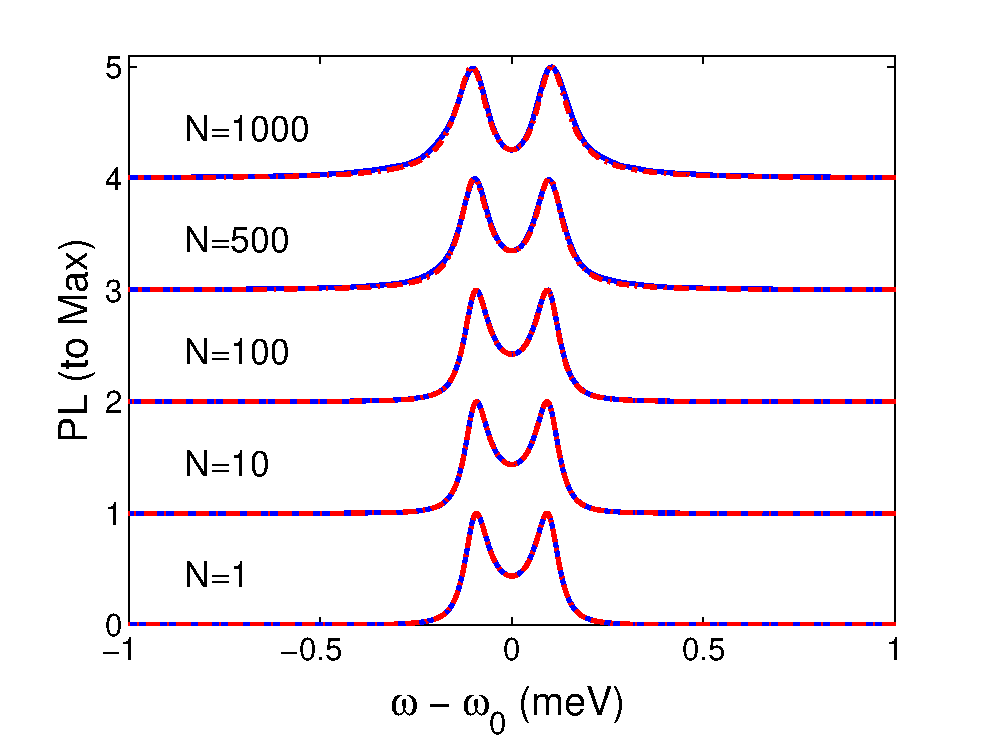
\includegraphics[width=.46\textwidth]{./Figs/GFT_ME_spec_str}}
     %\hspace{.1in}
     \subfigure[ ]{
          \label{fig:P_str}
                %\psfrag{ylabel}{$\frac{1}{\sigma}\frac{\rmd\sigma}{\rmd\ptsq}\gev^2$}
                %\psfrag{xlabel}{\small{$\ptsq\gev^2$}}
          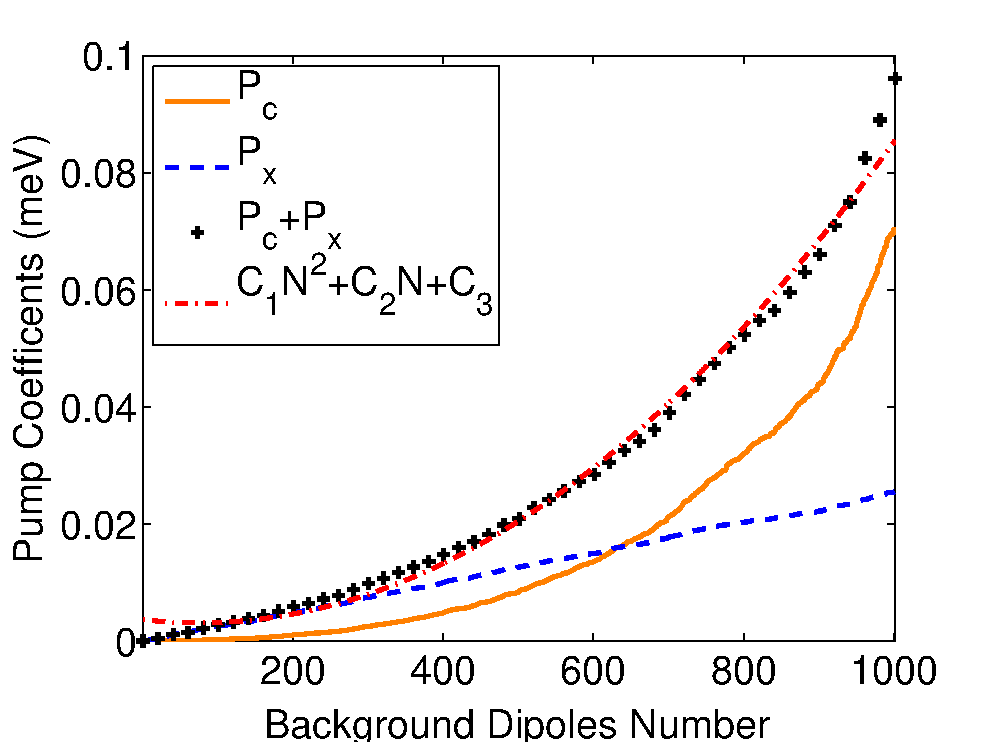
\includegraphics[width=.46\textwidth]{./Figs/P_str}}\\
     %\vspace{.1in}
%     \hspace{.1in}
     \subfigure[ ]{
           \label{fig:GFT_ME_spec_weak}
                %\psfrag{ylabel}{$\frac{1}{\sigma}\frac{\rmd\sigma}{\rmd\ptsq}\gev^2$}
                %\psfrag{xlabel}{\small{$\ptsq\gev^2$}}
           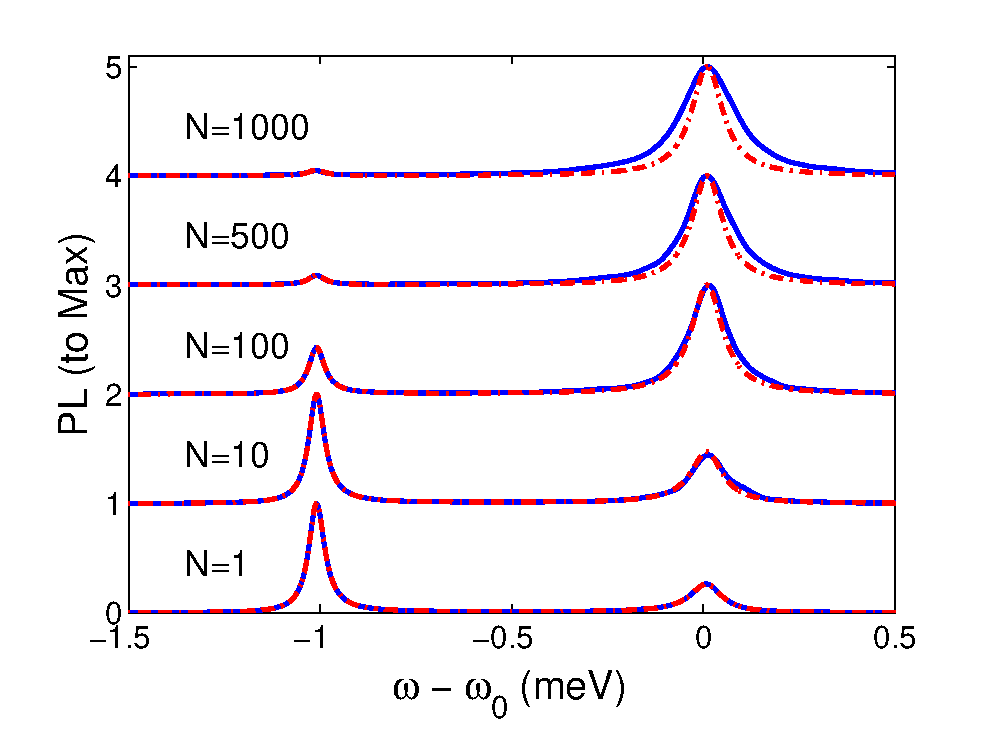
\includegraphics[width=.46\textwidth]
                {./Figs/GFT_ME_spec_weak}}
     \subfigure[ ]{
           \label{fig:P_weak}
                %\psfrag{ylabel}{$\frac{1}{\sigma}\frac{\rmd\sigma}{\rmd\ptsq}\gev^2$}
                %\psfrag{xlabel}{\small{$\ptsq\gev^2$}}
          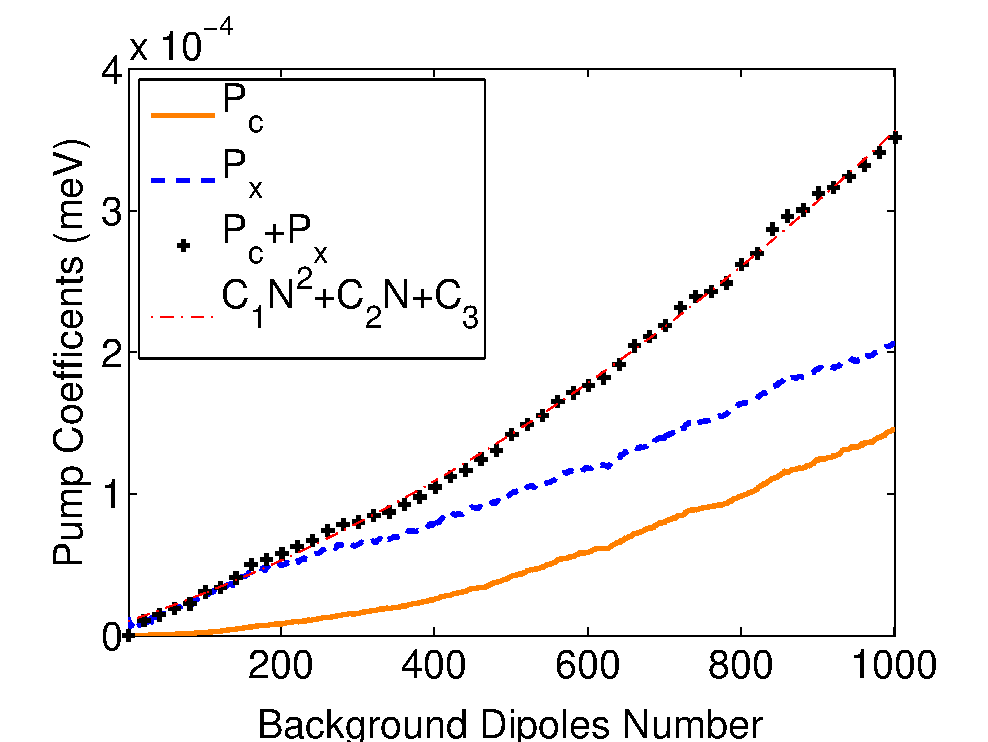
\includegraphics[width=.46\textwidth]{./Figs/P_weak}}
     \caption[Pumping as a tool for dipoles excitation.]{\textbf{  LS fit of ME model to GFT spectra as background dipoles number $N$ varies from $0$ to $1000$.} Both target dipole on-resonance (\subref{fig:GFT_ME_spec_str} and \subref{fig:P_str}) and off-resonance (\subref{fig:GFT_ME_spec_weak} and \subref{fig:P_weak}) cases are calculated. The GFT spectra (solid-blue curves in (a) and (c)) are averages of $400$ samples, each of which has up to $1000$ background dipoles Gaussianly distributed around the cavity resonance with a standard deviation of $\sigma=20$ meV. The best fit ME pumping coefficients $P_c+P_x$ show a good function form of $C_1N^2+C_2N+C_3$. See text for the detailed curve fitting procedure.}
     \label{fig:GFT_ME_fits}
\end{figure}

The curve fitting is performed as follows. First, we calculate the cavity spectra with $N$ dipoles ($N=1,2,\cdots,1000,\cdots$) based on the GF method with the parameters introduced in the last paragraph. Because the background dipoles are randomly distributed, and the spectrum relies on the resonance positions of the background dipoles, to obtain a robust statistical spectrum curve, we have averaged $400$ samples for each specific $N$. Next, we fit the exciton pumping parameter, $P_x$, to the $N=1$ spectrum of the GF method, by using the LSM with the ME spectrum formula (Equ.\eqref{S_ME}) with $P_c=0$. We can get a perfect fitting since the GF spectrum of $N=1$ is equivalent to the ME model described above with sole exciton pump (the target dipole is excited without any pump to the cavity mode)~\cite{Hughes2009}. Then, we use the best fitted $P_x$ and $P_c=0$ obtained above when $N=1$ as the initial values, and fit the next best pumping rates, $P_x$ and $P_c$, of the ME model to the GF spectrum of $N=2$, by using the LSM. We increase the $N$ one by one, and repeat the step above until $N$ is large enough. One may need to carefully adjust the iterative steps and tolerance of errors in the LSM setting to find the smoothly increasing pumping parameters of the ME model as $N$ increases. Our results are shown in Fig.~\ref{fig:GFT_ME_fits}.

We find that the two models fit very well in the linear region, and the pumping rates are correlated with the number of background dipoles with a clear physical meaning. As plotted in Figs.~\ref{fig:P_str} and~\ref{fig:P_weak}, for both on-resonance and off-resonance coupling cases, the pumping rate $P$ fits well a second order polynomial functions of $N$, which is $P=C_1N^2+C_2N+C_3$, where $C_1>0$, $C_2$ and $C_3$ are all constants. The exciton and cavity pumping rates, $P_x$ and $P_c$, are first-order and second-order functions of $N$, respectively. This fact can be interpreted as some excitations under pumping in cavities with homogeneously distributed photon emitters. If we suppose the average distance between photon emitters is given by $L=1/n$, where $n$ is the line density of emitters, and $\mathcal{S}$ is the luminescent area where there are $n^2$ excitons per unit area, then there are two interpretations of the second-order polynomial correlation relationship between pumping rates and background dipoles numbers: one is that, as the pumping power increases, the mean separation of excitons is not changed, but the luminescent area is enlarged linearly; the other interpretation is that, as the pumping power increases, the luminescent area is not changed, but the mean distance between excitons decreases linearly, or the number of excitons per unit area increases. The former interpretation may correspond to a large cavity with a limited or inhomogeneous pumping area, such as laser pumped molecular luminescence in a solution cavity; the latter one may correspond to a large pumping area with a limited cavity volume, such as optical pumped micropillar QDs single photon sources, where every QD could excite several excitons as pumping power is increased. Experimentally, it is possible to estimate how many color centers are excited in a microdisk cavity based on the scanning confocal image~\cite{Santori2010}, and the changing of the population of luminescent spots is consistent with the interpretations. Correspondingly, $P_c$ and $P_x$ both depend on the increasing number of excited dipoles coupled to the cavity, as both parameters are functions of $N$. All of the coupling between the background dipoles and the cavity are through the target dipole which has a stronger coupling strength to the cavity, since the the fitted parameters of $N$ depend on the relative position of the target dipole.

Notice that, since the number of physical luminescence centers, such as QDs in a semiconductor laser cavity or ions in a large liquid cavity, may not equal the actual number of excitons; the $N$ which we use throughout this paper refers to the number of excited excitons or dipoles. The cases of increasing $N$ can be realized by increasing the pump power or physically increasing the number of luminescent centers in all ways.

Although the two models fit well at first glance, the ME model in the one-exciton approximation fails to describe the inhomogenous broadening effect caused by the background dipoles (see the mismatch of the cavity spectra with $N>500$ in Fig.~\ref{fig:GFT_ME_spec_weak}). As the GF theory shows, depending on the distribution profile of the background dipoles, the spectrum of the ensemble coupled cavity can be reshaped into a non-Lorentzian envelope. The ME model fails in this case, because it cannot reflect the non-Lorentzian distribution of background dipoles.





\section{Cavity spectral behavior with an ensemble of background dipoles}

%As we discussed before, the ensemble of background dipoles can be treated as an entity, basically. So, the relative central resonance and effective optical moment (determined by the dipoles population) of the background dipoles will strongly affect the optical property. And a simplified few-dipole model can be used to analyze the cavity spectrum.


In section~\ref{PCcase}, we looked at the spectral behavior of a PC cavity with numbered background dipoles and one target dipole, and introduced some basic effects of changing the properties of optical cavities. In this section, we will move on to the discussion of dense dipoles coupled cavities. All results in this section are calculated using the GF method.



%\section{Spectral Behavior for Dense-dipole Coupled Cavities}\label{Onedipolecoupling}
%In this section, we will discuss a large amount of background dipoles coupled cavities.
Based on GF calculations, we find that, when all dipoles are far off the cavity resonance, the Purcell effect occurs and the cavity peak is repelled and narrowed. If there are some dipoles merged into the cavity peak, however, the cavity spectrum will be broadened and shifted, and the shift of the cavity peak center is affected by both the nearby and far-off-resonance dipoles in a complicated way. We discuss these two cases in detail.

\subsection{Cavities with Far-off-resonance Dipoles}
To show how far-off-resonance dipoles affect the cavity spectrum, we consider in a homogeneous field up-to $2000$ background dipoles which have an equal coupling strength and are off the cavity resonance. The same dipoles and cavity parameters as that of the last section are used, except for the dipole resonances. One example of the distribution of $2000$ dipole resonances is shown in Fig.~\ref{distr_wd0.5s0.1}. Now, let us increase the number of background dipoles from $1$ to $2000$, and average $200$ samples to get the mean values for the cavity shifts and widths as functions of dipole population. The cavity peak shift and the peak frequency of the dipoles ensemble shift are shown in Fig.~\ref{peakshift_wd0.5_detune_N}. Both exciton and cavity peaks are repelled from the center of the original $\Omega_d$ and $\omega_0$. The spectral shift is proportional to the effective coupling strength or $\sqrt{N}g_b$~\cite{Kimble1994}. The FWHM of the cavity spectrum is shown in Fig.~\ref{FWHMcav_2000wd0.5s0.1}. Note that the cavity spectrum will be narrowed down towards the individual dipole decay rate, which is consistent with the Purcell effect. In our case, when all dipoles are far off the cavity resonance, the photon is scattered among the background dipoles, and the decay time is increased, and hence the FWHM of the cavity spectrum is narrowed down. Moreover, both the cavity spectral shift and bandwidth curve match up the cases with defined dipoles when all dipoles share the same resonance and when there is only one dipole coupled to the cavity with a growing coupling strength. As has been discussed in Section~\ref{section:scenarios}, once the background dipoles have close resonances, the dipole ensemble is equivalent to a single effective dipole with a larger coupling strength of $\sqrt{N}g_b$ to the cavity.


\begin{figure}[htp]%[floatfix]
\centering
 \begin{tabular}{cc}
   \begin{minipage}[t]{0.44\linewidth}
   %\centering
    \subfigure[Dipole distribution with $\sigma=0.1$ meV and $\Delta\omega=-0.5$ meV.]{\label{distr_wd0.5s0.1}
    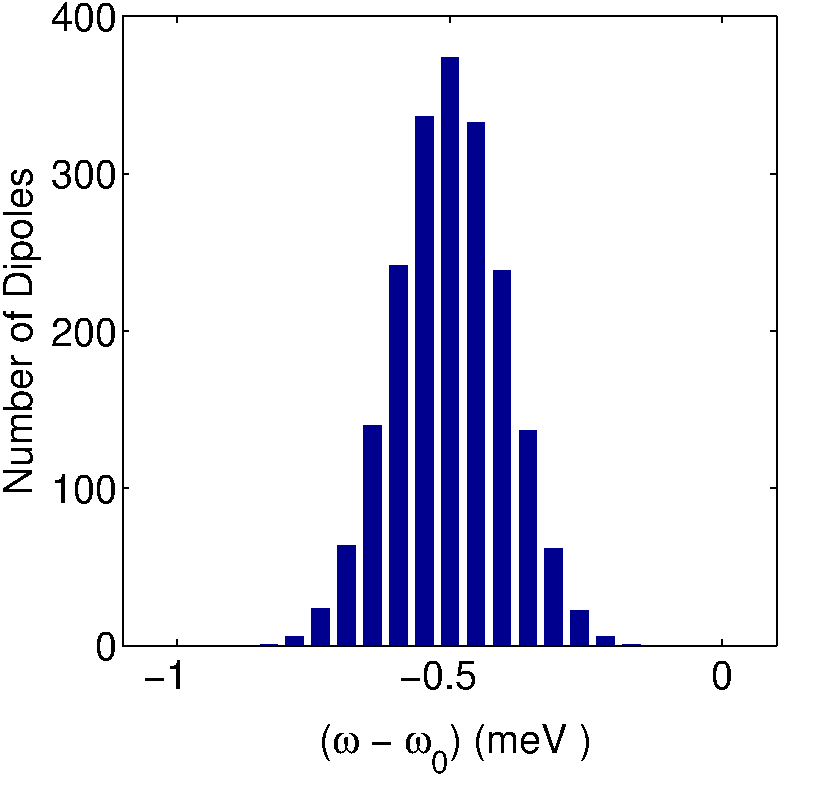
\includegraphics[width=1\textwidth,height=0.9\textwidth]{./Figs/distr_wd0dot5s0dot1}}
   \end{minipage} \qquad
   \begin{minipage}[t]{0.46\linewidth}
   \subfigure[FWHM of cavity peak as a function of $N$. ]{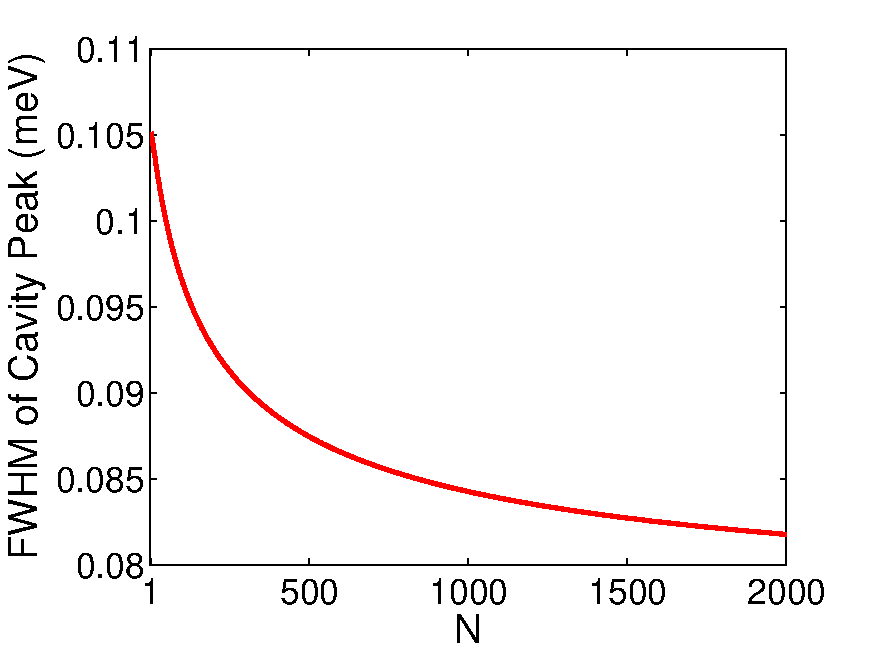
\includegraphics[width=1\textwidth,height=0.9\textwidth]{./Figs/FWHMcav_2000wd0dot5s0dot1}
    %\caption{\textbf{FWHM of cavity peak.} The QDs ensemble has a Gaussian distribution profile, centered at $-0.5$ meV left to cavity mode resonance, with standard deviation $\sigma=0,\,0.05,\,0.1$ meV. }
    \label{FWHMcav_2000wd0.5s0.1}}
   \end{minipage}
   \\
   %\begin{tabular}{cc}
   %\begin{minipage}[t]{0.34\linewidth}
   %\centering
   %\end{minipage}
  %&
  %\begin{minipage}
   \subfigure[Cavity and dipole peak shifts. ]{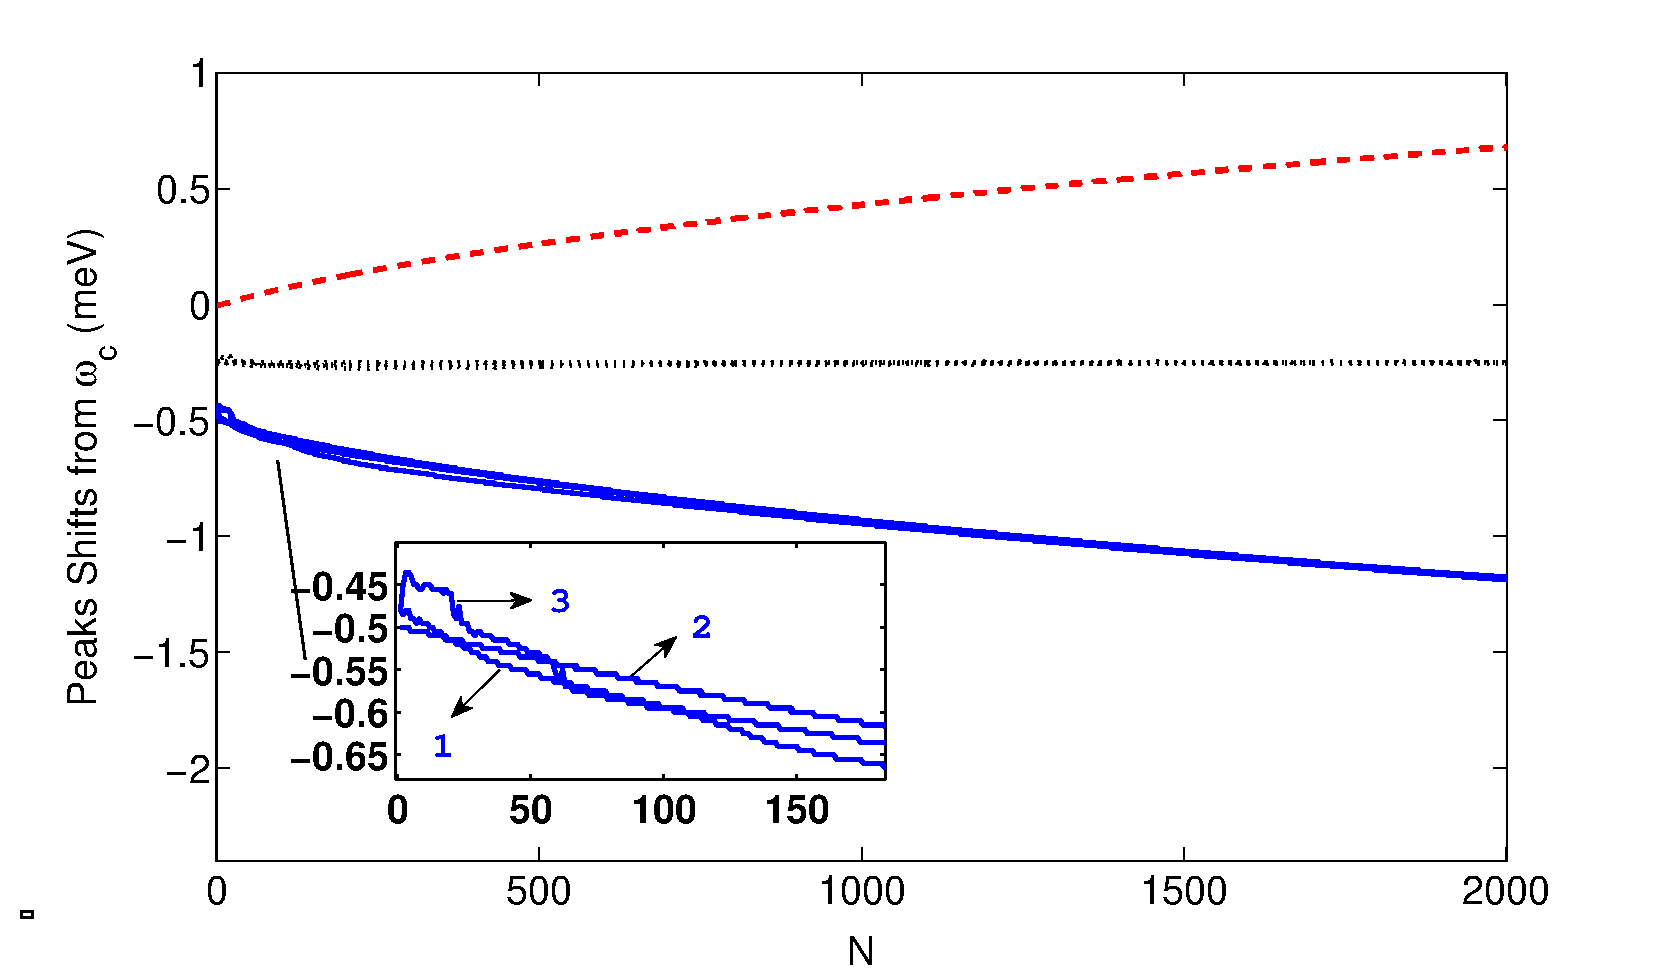
\includegraphics[width=0.56\textwidth,height=0.4\textwidth]{./Figs/peakshift_wd0dot5_detune_N}
    \psfrag{N}{Number of Dipoles}
   %\caption{\textbf{Repulsion effect.} The QDs ensemble has a Gaussian distribution profile, centered at $-0.5$ meV left to cavity mode resonance, with standard deviation $\sigma=0,\,0.05,\,0.1$ meV. }
   \label{peakshift_wd0.5_detune_N}}
  %\end{tabular}
  %\end{minipage}
  \subfigure[Dipole distribution with $\sigma=20$ meV and $\Delta\omega=-5$ meV.]{\label{wddistr_wdrand5s20_qd2000_stat100_2}
    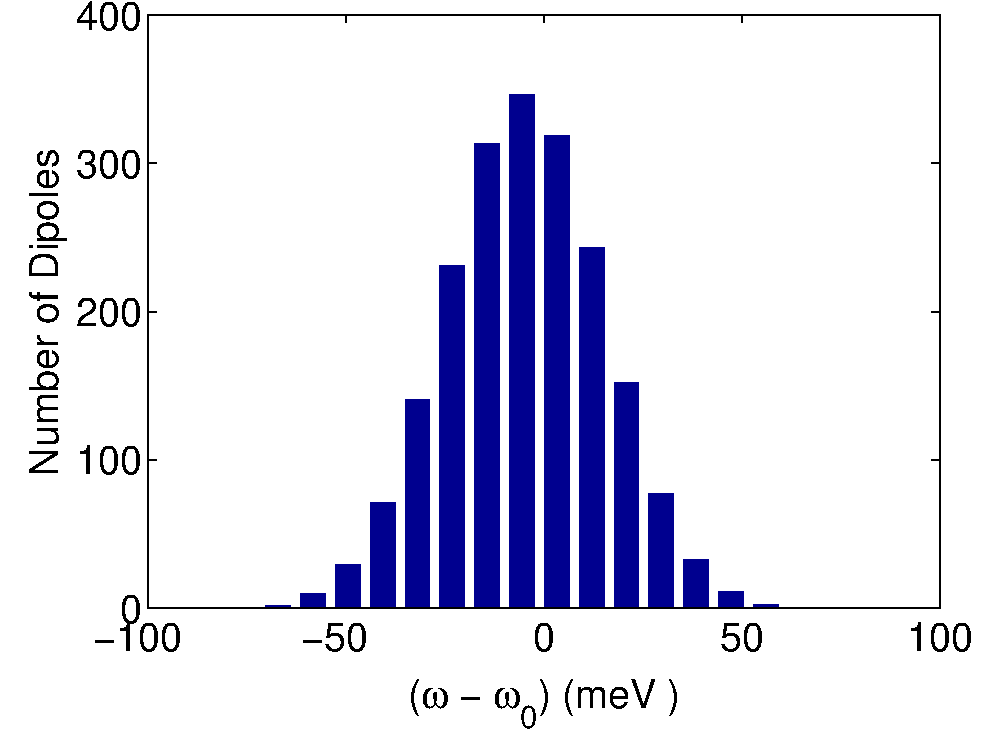
\includegraphics[width=0.40\textwidth,height=0.4\textwidth]
    {./Figs/wddistr_wdrand5s20_qd2000_stat200}}
  %&
  %\begin{minipage}[t]{0.49\linewidth}
  %\centering
  %  \subfigure[ ]{\includegraphics[width=1\textwidth,height=0.9\textwidth]{./Figs/PhaseChange_1wd0.5g0.02}
  %  \label{PhaseChange_1wd0.5g0.02}}
  %\end{minipage}
 \end{tabular}
\caption[Spectral modification of off-resonance ensemble.]{\textbf{  Off-resonance ensemble coupled cavity system.} \subref{distr_wd0.5s0.1} and~\subref{wddistr_wdrand5s20_qd2000_stat100_2} give two examples of the Gaussian distribution profile of dipole resonances with $\sigma=0.1$ meV and $\Delta\omega=-0.5$ meV, and $\sigma=20$ meV and $\Delta\omega=-5$ meV, respectively.
\subref{FWHMcav_2000wd0.5s0.1} shows the cavity width as a function of $N$.
The curve is averaged over $200$ samples of $\sigma=0.1$ meV dipoles sets.
\subref{peakshift_wd0.5_detune_N} shows that both the cavity (dashed red line) and dipoles (solid blue line) peak mean positions change as dipoles number $N$ increases. Inset is a magnified segment of dipole peak position,
where label 1 corresponds to the single-dipole case and equivalent to the $\sigma=0$ case,
label 2 shows the $\sigma=0.05$ meV case,
and label 3 shows the $\sigma=0.1$ meV case.
The difference between the curves is small.}
%\subref{PhaseChange_1wd0.5g0.02} the phase diagram of GF of a single-dipole coupled cavity system with $\Omega_d=\omega_0-0.5$ meV, and $g=0.02$ meV. }
\end{figure}

% phase changing
%Notice that there are some beats in the FWHM changing with respect to the number of dipoles (inset of Fig.~\ref{FWHMcav_2000wd0.5s0.1}). This can be explained by analogically introducing the concept of phase angle, $\theta$, which is commonly used in RLC circuit signal analysis to describe wave beating.

%For a RLC circuit, the tangent of a phase angle is defined by $\tan\theta=\frac{L-C}{R}$ and indicates the power fluctuation caused by phase difference between the current and the voltage~\cite{Neamen2001}, where $L$ is the inductance of the load, $C$ is the capacitance, and $R$ is the resistance of a circuit. Researchers have shown that some cases of dipole-cavity interactions can be equivalent to some simple RLC circuits~\cite{Greffet2010}. And the far-off-resonance case we are discussing is basically a one-dipole coupled cavity system, which has an equivalent RLC circuit. Therefore, we can similarly bring the signal analysis method into our ensemble-cavity coupled system by identifying corresponding quantities of resistance, inductance and capacitance of the equivalent RLC circuits for our case. Following the equivalent circuits method discussed in Ref.~\onlinecite{Greffet2010}, for ensemble coupled cavities, one can analogically define the phase angle as the ratio of the imaginary part and the real part of the field strength that determines the spectrum.
%The only difference between optical system and electronic circuits is that the phase angle becomes a tensor for various optical components.
%For instance, in a single-dipole coupled system, we can obtain the $ij$-component of corresponding phase angle tensor by
%\begin{equation}
%\label{phase}
%\begin{split}
%\tan\theta_{ij} =& \frac{imag(E_i(\br))}{real(E_j(\br))}\\
%=& \frac{-\omega\left[\Gamma_d (\omega^2-\Omega_d^2)+\Gamma_i (\omega^2-\Omega_d^2)\right]}{(\omega^2-\omega_j^2) (\omega^2-\Omega_d^2)-\omega^2 \Gamma_j \Gamma_d-4g^2 \omega_j \omega},
%\end{split}
%\end{equation}
%where $i,j=x,y,z$ label different mode components of the cavity, $\omega_j$ indicates the $j$-th mode in orthogonal directions, and $\Omega_d$ and $\Gamma_d$ are the resonance and decay rate of the dipole. For single-direction polarized cases with single cavity mode, the phase angle tensor is reduced to a scalar ($i=j$). In Fig.~\ref{PhaseChange_1wd0.5g0.02} for a given $g$, we can see that at exciton and cavity resonances, the phase approaches to $\pm \pi/2$, which means the electrical field has almost only the imaginary part; while at frequencies far away from resonances, the phase angle approaches to $0$, which corresponds to a pure real electrical field. Generally, the imaginary part of the field usually has a Lorentzian lineshape, and the mode of the real part of the field is basically outside of the imaginary part. Recalling that the phase angle determines the relative magnitude of the real and imaginary parts, therefore, the tangent of the phase angle can reflect the linewidth of the cavity spectrum.

%As shown in the equation above, once the bare cavity mode is given, the phase angle is determined by the central position, the width of the dipole peak and the coupling strength between the dipole source and the optical cavity (determined by $\sqrt{N}g_b$, in our case). Consequently, as $N$ or $g_b$ increases, the spectrum width will change with fluctuating beats, indicated by Equ.\eqref{phase} as a high-order fraction of $g$ and $\omega$. It shows that as we increase the number of background dipoles, the ``phase angle'' changes periodically. If $N$ is small, all dipoles pull down the width of the cavity spectrum; when the cavity spectrum has a width approximate to the dipole's decay rate, the newly added background dipoles give considerable beating effect on the width of the cavity spectrum, just like a ``phase'' changes in a circle.  The variance of the beating curves caused by the random distribution of the background (indicated by $\sigma$) is negligible if the dipoles are far away from the cavity resonance.
%To show a simple example in the case of scenario one, one can randomly excite many dipoles with a Gaussian distribution profile which is far away from the cavity spectral envelope, as shown in Fig.~\ref{distr_wd0.5s0.1}, and observe the spectrum width of the cavity. The result is shown in Fig.~\ref{FWHMcav_2000wd0.5s0.1}, where the average cavity peak narrows down with a small fluctuation (see the inset plot).
%The author would like to address that this fluctuation comes from the complexity of phase angle indicated in Equ.\eqref{phase}, because the result is robust to the random distribution of background dipoles and the bandwidth curve matches up the cases with defined dipoles when all dipoles share the same resonance and when there is only one dipole coupled to the cavity with a growing coupling strength.

%In the same way, one can find that two-dipole coupled cavity system has similar properties. The corresponding collective spectral behavior of scenario two will be discussed later with various $\Omega_d$, $\sigma$, $N$ and $g_b$.


%Considering the discussion in the theory of GF on effective coupling strength of background dipoles,
Therefore, coupling a large number of off-resonance dipoles can be used to enhance the Purcell effect for cavity optical property control. However, in most cases, there is at least one dipole close to or on resonance in the cavity. We will discuss these cases in the following part.


\subsection{Cavities with On-resonance Dipoles}
As discussed in the discrete dipoles case of section~\ref{PCcase}, the dipoles close to the cavity resonance can have a great influence on the cavity spectrum. In this section, we assume there is always a target dipole on resonance with the cavity, while there are a large number of background dipoles randomly distributed in a Gaussian profile in a large range.


Through sampling and simulating, it was found that the relative coupling strength and position between the target dipole and background dipoles, as well as the relative coupling strength of the target dipole to the cavity decay rate, affect the cavity's optical properties dramatically, especially for the behavior of the cavity peak shift. However, once there is a target dipole merged in the cavity peak, the cavity spectrum is statistically broadened as the number of dipoles increases. We will discuss the case when the target dipole has equally relative strong coupling strength to the background dipoles in the following paragraphs. To better understand how the target dipole affects the cavity spectrum and how the background dipoles affect the target dipole, we simultaneously present both the total cavity and the target dipole spectra, labeled as $S^{total}$ and $S^{t}$, respectively.

% Case 1: the target dipole has the same coupling strength as the background dipoles do.

Now, we first let all dipoles have the same coupling strength to the cavity, that is $g_t=g_b=g$. As the coupling strength increases, both the broadening and repulsion effects will be enhanced, as long as there are dipoles falling into the cavity spectrum region. The results of cavity width and shift with $g=0.02$ meV and $g=0.04$ meV are shown in Figs~\ref{fwhm_wdrand5s20_E0.2-0.4_qd2000_stat200} (a) and (b), respectively. Note that I have used the same set of parameters as the last section, except now that $\Delta\omega=-5$ meV and $\sigma=20$ meV (reference to Fig.~\ref{wddistr_wdrand5s20_qd2000_stat100_2} for the $2000$-dipole distribution at $\Delta\omega=0$ meV). As we have discussed in the last part of section~\ref{PCcase}, $g=0.04$ meV is close to the threshold to give a doublet, so the initial spectral width with the target dipole on-resonance is close to $0.1$ meV, which is the decay rate of the cavity; while for $g=0.02$ meV, the on-resonance target dipole gives the Purcell effect and the FWHM of the initial spectrum solely with the target dipole is close to $\Gamma_d=0.05$ meV and less than $\Gamma_c=0.1$ meV. One sample spectrum with a different number of background dipoles is shown in Fig.~\ref{spec_wdrand5s20_E0.2_qd2000_stat200_sam32}.

%\begin{figure}[H]%[floatfix]
%\centering
%\begin{center}
% \begin{minipage}[t]{0.49\linewidth}
%   %\centering
%    \subfigure[]{\label{distr_wd0.5s0.1}
%    \includegraphics[width=1\textwidth,height=1.0\textwidth]{./Figs/distr_wd0.5s0.1}}
%   \end{minipage}
%   \begin{minipage}[t]{0.49\linewidth}
%    \subfigure[]{\label{wddistr_wdrand5s20_qd2000_stat100_2}
%    \includegraphics[width=1\textwidth,height=1.0\textwidth]
%    {./Figs/wddistr_wdrand5s20_qd2000_stat200}}
%   \end{minipage}
%\end{center}
%\caption[2000-dipole distribution with a Gaussian profile.]{\textbf{Average dipole distribution over 200 samples, each with 2000 dipoles.} The shown dipoles ensemble has a Gaussian distribution, centered at 5 meV left to cavity mode resonance, with standard deviation $\sigma=20$ meV. }
%%    %\includegraphics[width=0.23\textwidth]{fwhmG_wdrand5-50s20_E0.2_qd2000_stat100_0}
%%\end{center}
%%\caption{\textbf{FWHM of Green's functions as dipoles ensemble centered at %$\omega_0-5$ meV, $\omega_0-10$ meV, $\omega_0-20$ meV and $\omega_0-50$ meV %(from top to bottom).} All ensemble samples share the same $\sigma=20$ meV. %Ensemble centered at plus side to $\omega_0$ has similar behaviour according %to their spectral distance to $\omega_0$. Here, $N=0$ means there is no other %dipoles except for one on-resonance dipole. }
%%    \label{fwhmG_wdrand5-50s20_E0.2_qd2000_stat100_0}}
%\end{figure}


\begin{figure}[htp]%[floatfix]
\centering
\begin{center}
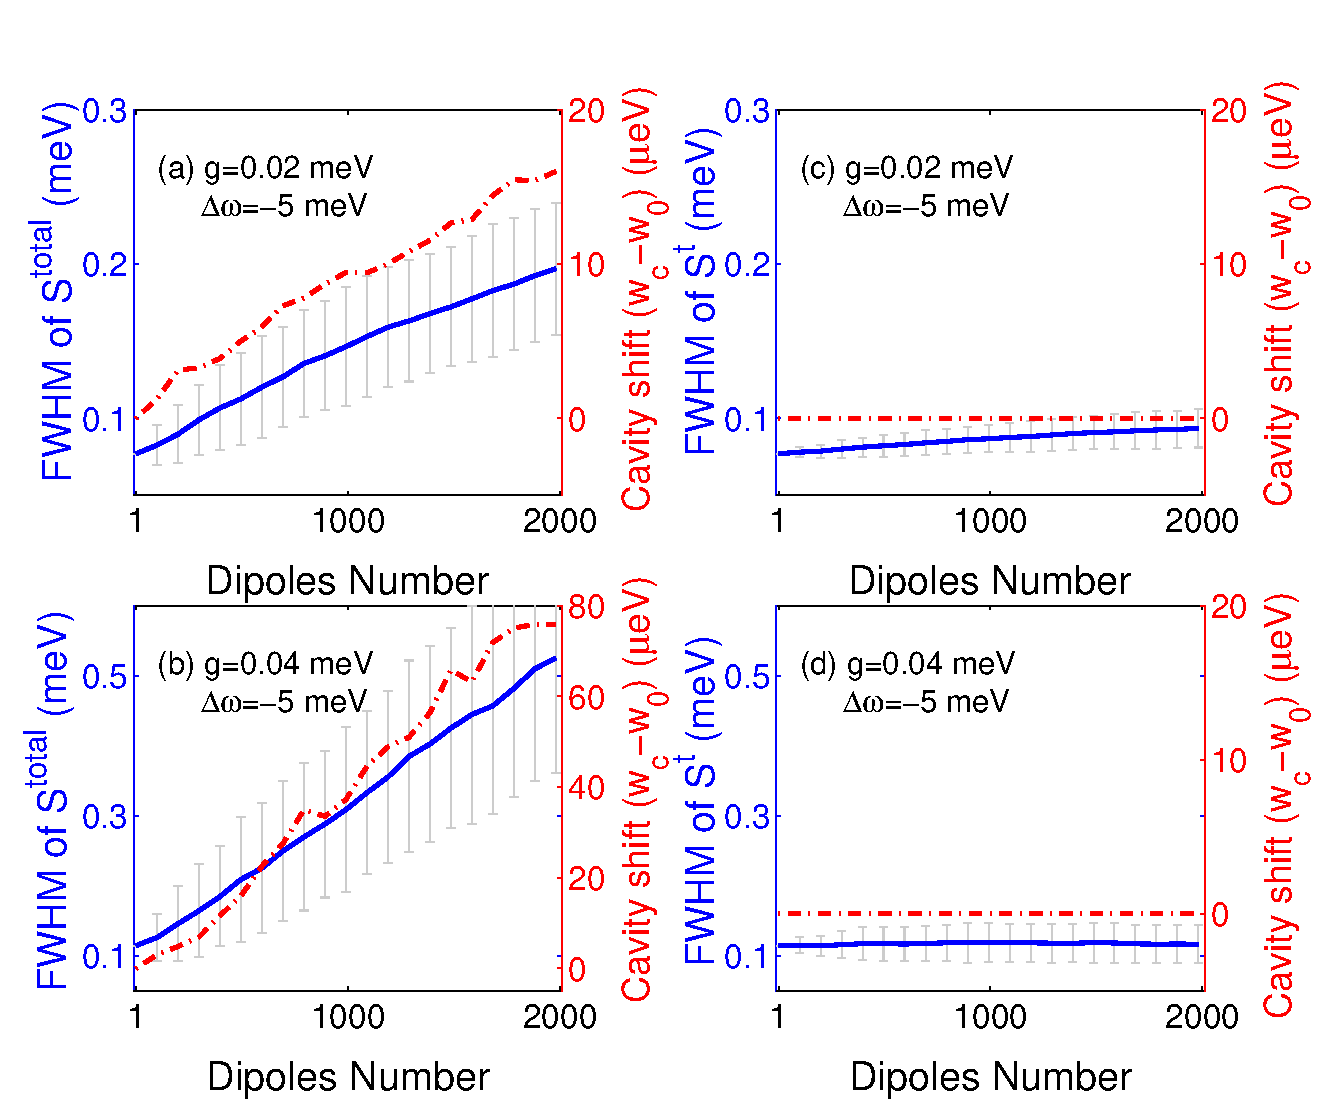
\includegraphics[width=12cm]{./Figs/fwhm_wdrand5s20_E0dot2-0dot4_qd2000_stat200}
\end{center}
\caption[Spectral modification by pure background dipoles.]{\textbf{  FWHMs (blue solid line) and peaks shifts (red dashed line) of cavity and dipole 1 spectra with a dipoles ensemble of the same coupling strength $g$.} Curves are averaged over 200 samples with the same distribution function. The gray vertical bars around blue line demonstrate the standard deviation of the FWHM obtained from 200 statistical samples. The cavity resonance shift is referenced to the bare cavity resonance with a high frequency shift as positive shift. (a) and (c) show the FWHM and peak shifts of the total cavity and QD 1 spectra respectively, with $g=0.02$ meV; (b) and (d) are with $g=0.04$ meV. Other parameters used are: $\Gamma_c=0.1$ meV, $\Gamma_d=0.05$ meV, bare cavity resonance $\omega_c=792.25$ meV, central angular frequency shift of dipoles ensemble $\Delta\omega=-5$ meV. }
\label{fwhm_wdrand5s20_E0.2-0.4_qd2000_stat200}
\end{figure}

Notice that the target dipole sitting in the cavity peak in the frequency domain can be slightly affected by the background dipoles, if the coupling strength is weak. In our case, the spectral width and shift of the target dipole spectra, $S^t$, are shown in Fig.~\ref{fwhm_wdrand5s20_E0.2-0.4_qd2000_stat200} (c) and (d). From the figure, one can find that $S^t$, the target dipole spectral peak, is broadened from $0.05$ meV$=\Gamma_d$ as $N$ grows, if the coupling strength is so weak ($g=0.02$ meV) that the cavity cannot screen the interaction with the background dipoles outside, unless the decay rate of the target dipole is comparable with the cavity decay rate; if the coupling strength is large enough, however, the cavity can well screen the target dipole from interacting with the background dipoles and stabilize $S^t$ at $0.1$ meV$=\Gamma_c$. In contrast, the peak position of the target dipole is stabilized at the original position on average, once the target dipole is sitting in the cavity peak. This phenomenon is valid for $g_t\leq g_b$.

Compared with the broadening and shifting of the cavity peak,
the target dipole peak change is so small that one can conclude the broadening and shifting of the cavity peak mainly comes from the nearby background dipoles.
%The more background dipoles merged into the cavity peak, the broader the cavity peak will become.



%the changes of $S^t$ is very small. So, the broadening and shifting effects are mainly generated by the background dipoles in an inhomogeneous way, as discussed in the last section.
%In our dipoles-cavity interaction picture, the on-resonance target dipole couples to the cavity to give an initial spectrum, then other background dipoles interact with the pre-coupled system. Only when there are dipoles close to the cavity resonance yet not on resonance, can the cavity spectrum be broadened by merging neighboring peaks in-homogeneously, or shifted by neighboring oscillators according to their repulsion strength. One sample of spectra with different number of background dipoles are shown in Fig.~\ref{spec_wdrand5s20_E0.2_qd2000_stat200_sam32}.

\begin{figure}[htp]%[floatfix]
\centering
\begin{center}
%\psfrag{PL}{$PL (to Max)$}
%\psfrag{omega-omega}{$\omega-\omega_c (meV)$}
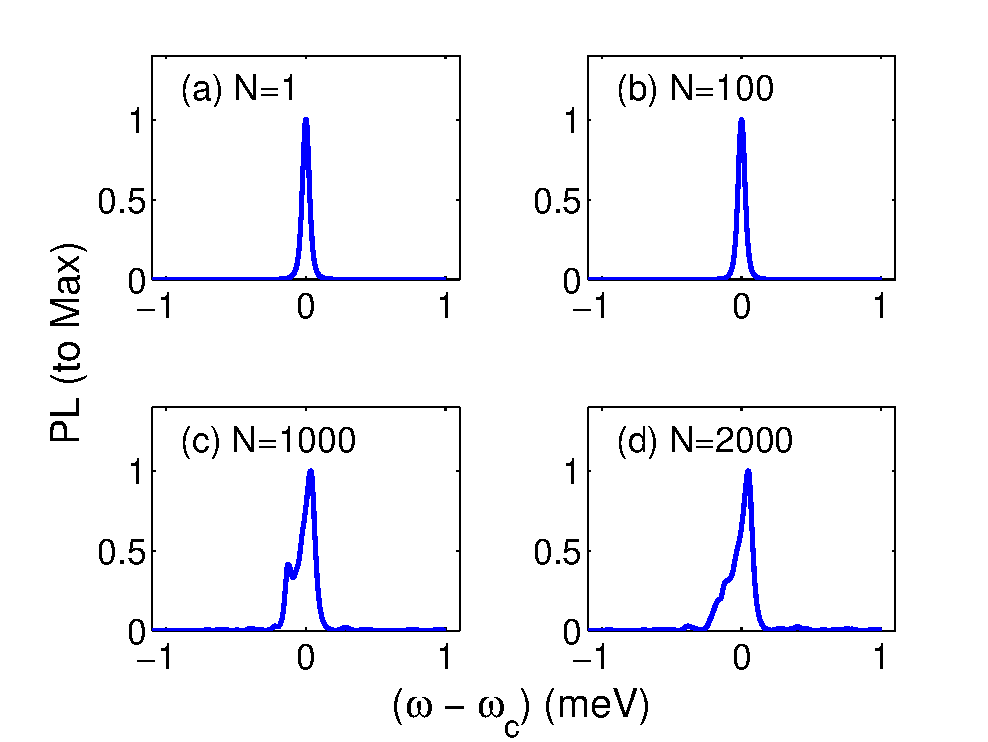
\includegraphics[width=12cm]{./Figs/spec_wdrand5s20_E0dot2_qd2000_stat200_sam1} %spec_wdrand5s20_E0.2_qd2000_stat200_sam32.eps
\end{center}
\caption[Spectra samples for $N$ background dipoles coupled cavity]{\textbf{  Cavity spectra of one set of dipole samples with various background dipole populations $N$.} As $N$ is large, the shape of the cavity spectrum is changed dramatically. We used $\Delta\omega=-5$ meV and $\sigma=20$ meV.}
\label{spec_wdrand5s20_E0.2_qd2000_stat200_sam32}
\end{figure}


\vspace{\baselineskip}
% Case 2: the target dipole has greater coupling strength than the background dipoles do.
We now discuss the spectral behavior if $g_t>g_b$. In our sampling calculations, we always make $g_b=\frac{1}{2}g_t<\Gamma_d=0.05$ meV. The other parameters for the cavity and the individual dipole are the same as before. $g_t$ in both the weak coupling regime and close to the strong coupling regime will be discussed. We also found that the positions of the background dipoles, or the number of dipoles close to the cavity resonance affects the spectral behavior greatly. We will also discuss this effect.

\begin{figure}[H]%[floatfix]
\centering
\begin{center}
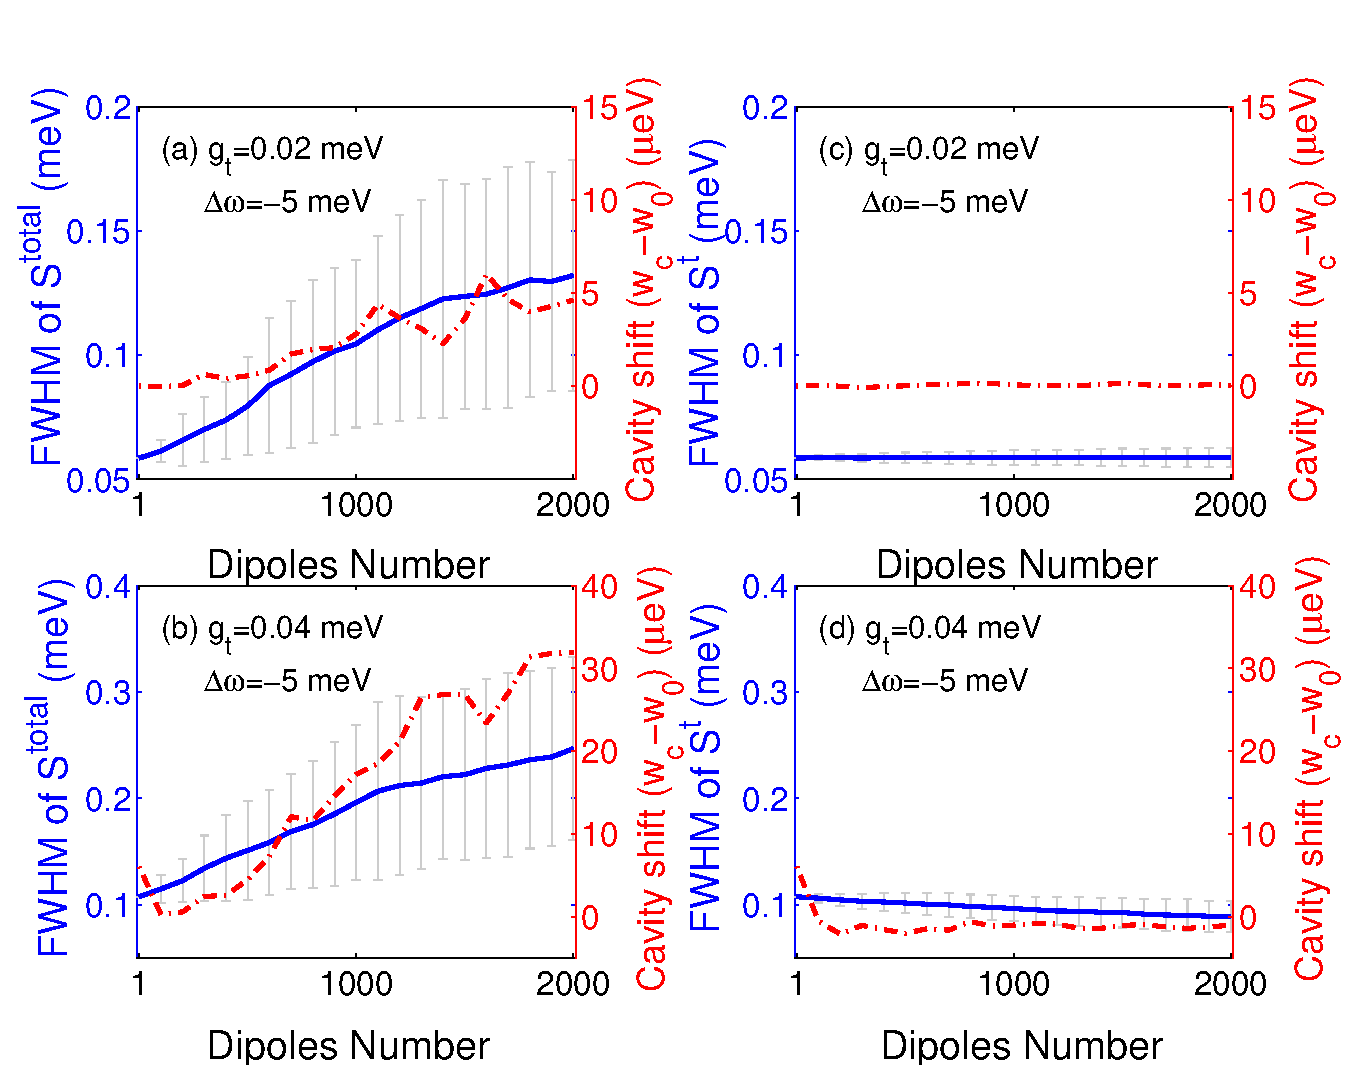
\includegraphics[width=12cm]{./Figs/fwhm_wdrand5s20_gt0dot2-0dot4_qd2000_stat200}
\end{center}
\caption[Spectral modification of a cavity with a target dipole and an ensemble.]{\textbf{  FWHMs (blue solid line) and peak cavity resonance shifts (red dashed line) of cavity mode spectrum for dipole ensemble with $g_b=0.5g_t$.} All curves are averaged over 200 samples randomly generated under the same distribution function. The vertical gray bars around the blue line illustrates the standard deviation of the FWHM obtained from the 200 statistical samples. The cavity resonance shift is referenced to the bare cavity resonance with high frequency shift as positive shift. (a) and (c) show the respective total and target dipole spectral FWHMs and peak shifts with $g_t=0.02$ meV; (b) and (d) are for $g_t=0.04$ meV. Other parameters used to generate this graph were: $\Gamma_c=0.1$ meV, $\Gamma_{d}=0.05$ meV, bare cavity resonance $\omega_c=792.25$ meV, central angular frequency shift of dipoles ensemble $\Delta\omega=-5$ meV. }
\label{fwhm_wdrand5s20_gt0.2-0.4_qd2000_stat200}
\end{figure}

\begin{figure}[htp]
\centering
\begin{tabular}{cc}
  \subfigure[ ]{
    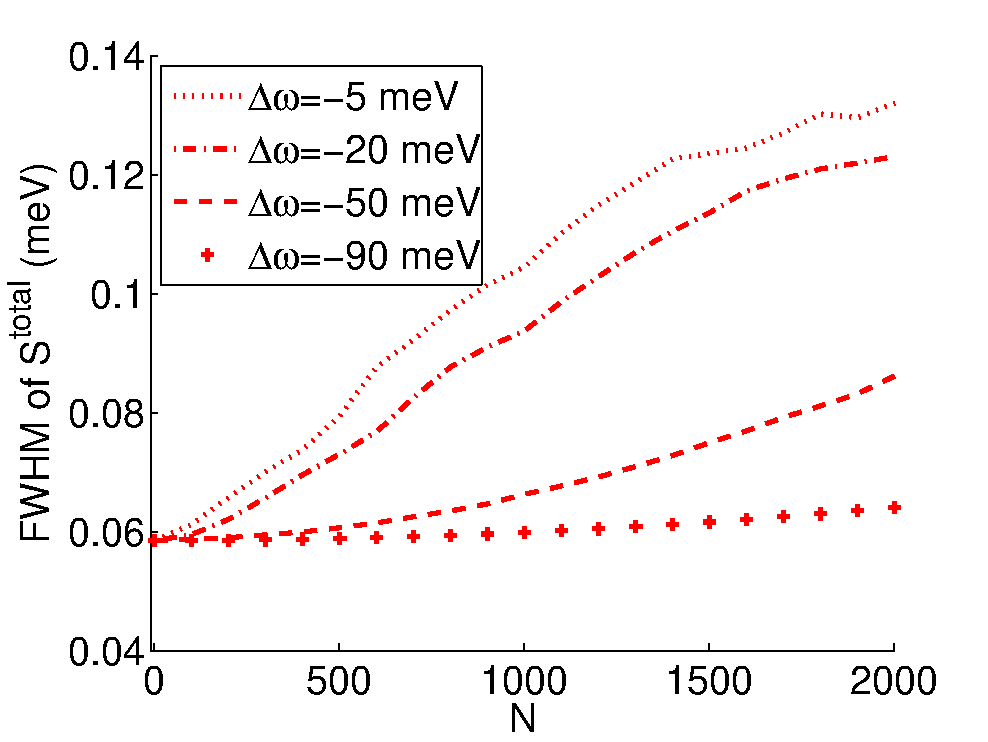
\includegraphics[width=0.46\textwidth]{./Figs/Stotalfwhm_wdrand5-90s20_gt0dot02b0dot5_qd2000_stat200}
    \label{Stotalfwhm_wdrand5-90s20_gt0.02b0.5_qd2000_stat200}}
 &
  \subfigure[ ]{
    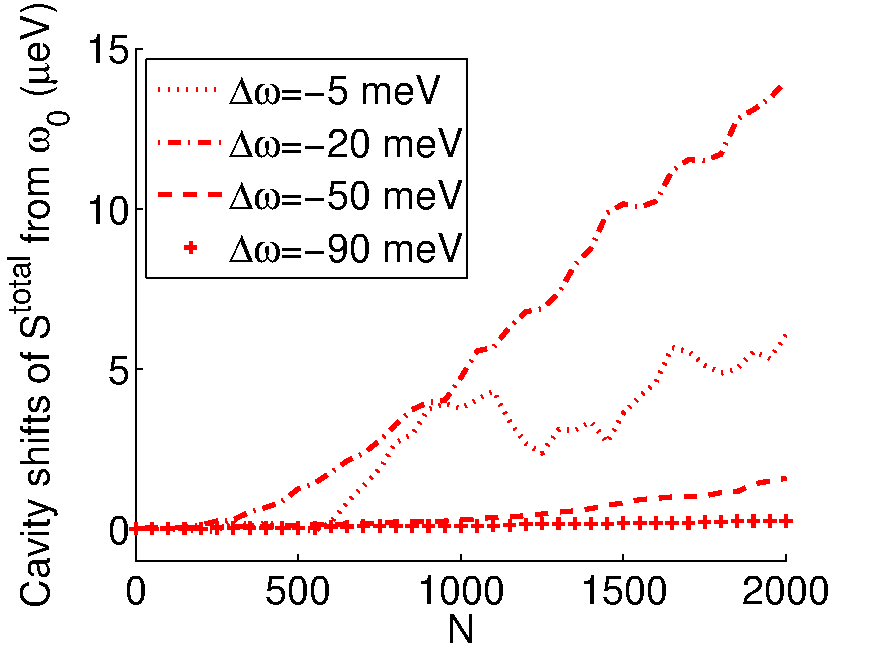
\includegraphics[width=0.46\textwidth]{./Figs/Stotalshift_wdrand5-90s20_gt0dot02b0dot5_qd2000_stat200}
    \label{Stotalshift_wdrand5-90s20_gt0.02b0.5_qd2000_stat200}}
%  \\
 \end{tabular}
\
  \begin{tabular}{cc}
  \subfigure[ ]{
    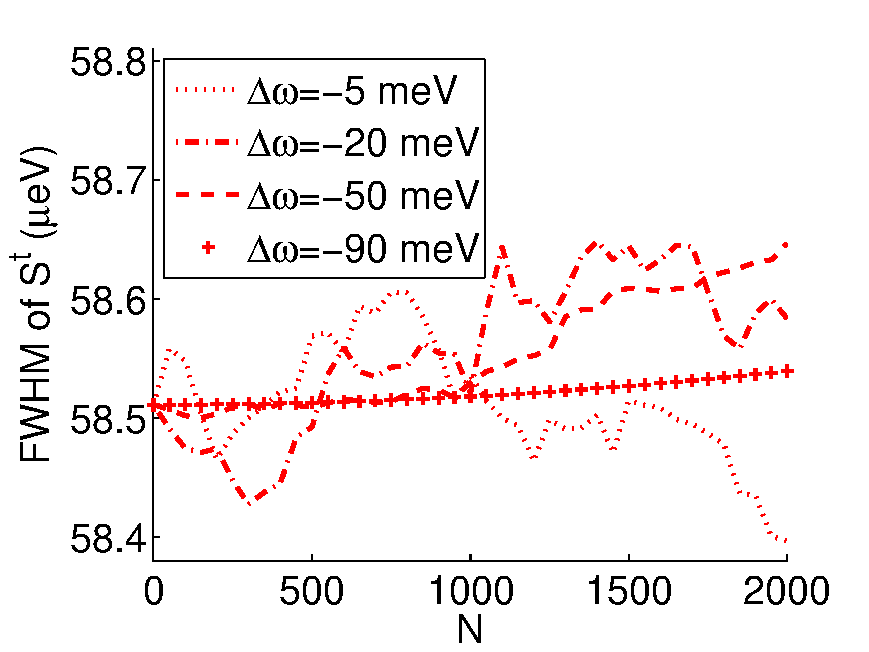
\includegraphics[width=0.46\textwidth]{./Figs/Stfwhm_wdrand5-90s20_gt0dot02b0dot5_qd2000_stat200}
    \label{Stfwhm_wdrand5-90s20_gt0.02b0.5_qd2000_stat200}}
  &
  \subfigure[ ]{
    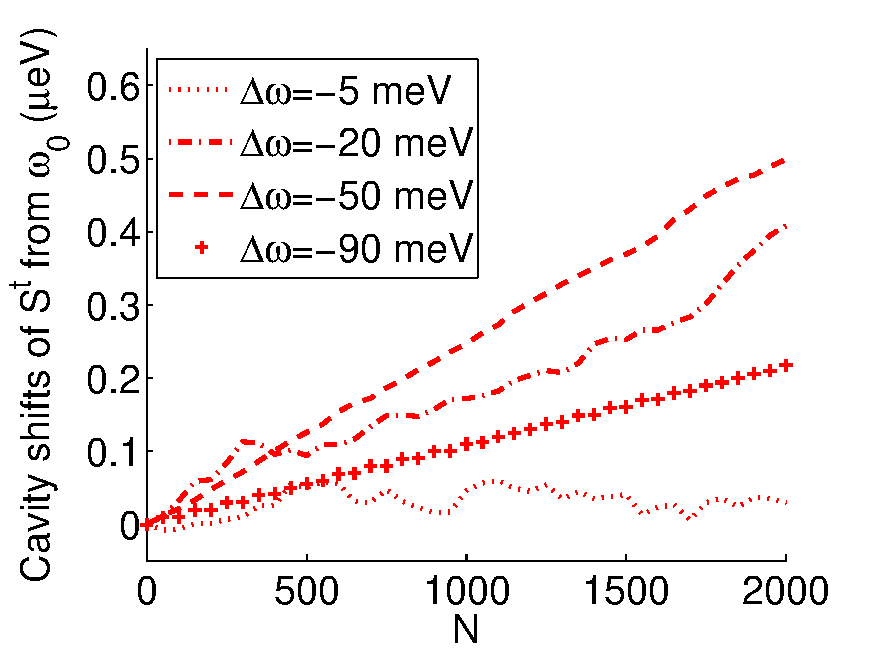
\includegraphics[width=0.46\textwidth]{./Figs/Stshift_wdrand5-90s20_gt0dot02b0dot5_qd2000_stat200}
    \label{Stshift_wdrand5-90s20_gt0.02b0.5_qd2000_stat200}}
\end{tabular}
\caption[Modification effect of different $\Delta\omega$ when $g_t=0.02$ meV.]{\textbf{FWHMs and shifts of the cavity and the target dipole spectra with different $\Delta\omega$ but with the same $g_t=0.02$ meV.} \subref{Stotalfwhm_wdrand5-90s20_gt0.02b0.5_qd2000_stat200} and \subref{Stotalshift_wdrand5-90s20_gt0.02b0.5_qd2000_stat200} show the total spectra are greatly broadened and shifted with the effect of close dipoles. The fluctuation feature is interpreted in the text, when $\Delta\omega$ is small. \subref{Stfwhm_wdrand5-90s20_gt0.02b0.5_qd2000_stat200} and \subref{Stshift_wdrand5-90s20_gt0.02b0.5_qd2000_stat200} show the similar effects on the target dipole spectra, but with a screening effect from the cavity peak. To demonstrate the phase retardation, we have averaged 600 samples for the four subfigures, and used a frequency domain resolution of $0.01\,\mu$eV for \subref{Stfwhm_wdrand5-90s20_gt0.02b0.5_qd2000_stat200} and \subref{Stshift_wdrand5-90s20_gt0.02b0.5_qd2000_stat200}, and $0.075\,\mu$eV for \subref{Stotalfwhm_wdrand5-90s20_gt0.02b0.5_qd2000_stat200} and \subref{Stotalshift_wdrand5-90s20_gt0.02b0.5_qd2000_stat200}. }
\label{fwhm_shift_gt0.02_dw}
\end{figure}

If the coupling strength of the target dipole is small, the cavity mode only provides a weak screening effect on the target dipole, and the background dipoles can provide weak repelling and broadening effects on both the cavity and target dipole spectra. One example with $g_t=0.02$ meV and $\Delta\omega=-5$ meV is studied. The FWHMs and shifts of the cavity and target dipole spectra are shown in Fig.~\ref{fwhm_wdrand5s20_gt0.2-0.4_qd2000_stat200} (a) and (c), in which the error bars indicate the sampling variance of FWHM. Compared with Fig.~\ref{fwhm_wdrand5s20_E0.2-0.4_qd2000_stat200}, there are two features worth mentioning. One is that the width of the target dipole spectrum is basically stabilized around $0.058$ meV, which is the width for the one-dipole coupled system (corresponds to $N=1$). If we shift the central position of the background dipole ensemble, various FWHM curves occur to indicate there are complex interactions between the background dipoles and the target dipole (see Figs.~\ref{Stotalfwhm_wdrand5-90s20_gt0.02b0.5_qd2000_stat200} and~\ref{Stfwhm_wdrand5-90s20_gt0.02b0.5_qd2000_stat200}). For example, if $\Delta\omega=-20$ mev, the FWHM of the target dipole can be narrower than the initial FWHM at $N=1$. This may be explained by noting that, there are dramatically more dipoles on the lower frequency side than the higher frequency side of the target dipole (reference to Fig.~\ref{wddistr_wdrand5s20_qd2000_stat100_2}) which gives a much stronger differential narrowing effect (the unbalanced repulsion effect on both half-leaves of the peak) than the broadening effect caused by the dipoles merged in the target dipole peak. Because the cavity peak is much wider than the target dipole peak, the broadening effect still dominates the spectral behavior for the cavity peak. When the frequency distribution center of the background dipoles is at other positions, the differential narrowing effect is weak and the broadening effect dominates the spectral behavior of the peaks, which is mainly determined by the number of dipoles merged in the corresponding peak. Also notice that the fluctuations in Fig.~\ref{Stfwhm_wdrand5-90s20_gt0.02b0.5_qd2000_stat200} are caused by the randomness of sampling and are within the order of $1\%$ of the dipole decay rate.

The second feature of the spectra is that there are phase retardation in the spectral shift curves. As you can see in Figs.~\ref{Stotalshift_wdrand5-90s20_gt0.02b0.5_qd2000_stat200} and~\ref{Stshift_wdrand5-90s20_gt0.02b0.5_qd2000_stat200}, both cavity peak and target dipole peak are shifted to the high frequency side, which indicates the repulsion effect from the background dipoles on the low frequency side, but there are some fluctuations in both curves. One can further notice that there is a retardation between the target dipole shift and cavity shift. Let us look in the peak shift curves of $\Delta\omega=-20$ meV, for example. Before $N=300$, the target dipole peak is first repulsed to the high frequency side of its original position, while the cavity peak is almost stabled at the origin; at $N=500$, the target dipole is then shifted to the low frequency side a little, while the cavity is on the high frequency side of the origin; as $N$ increases, both curves are shifted to the high frequency side with fluctuations. The amplitude of the fluctuations when $N>500$ are affected by the calculation resolution once the number of statistical samples is large, but the trend of the peaks' movements is regardless of the calculation resolution. This phenomenon reflects the interaction and ``energy'' transmission process as the number of background dipoles grows: at the beginning, background dipoles are more likely to interact with the target dipole, and the target dipole can repel the cavity peak greatly, as the coupling strength indicates; as the number or the effective coupling strength of background dipoles grows, the background dipoles can greatly transfer ``energy'' to the cavity until the cavity is strong enough to suppress the shift of the target dipole and establishes a new balance of peaks' moving. Note that, in weak coupling cases, the shifts of each peak are small; since the cavity peak is wider than the target dipole peak, the differential repulsion to the cavity is larger than that to the target dipole, and hence the cavity peak moves faster than the target dipole peak does as $N$ increases.




% g_t=0.04 meV
\begin{figure}[H]%[floatfix]
\centering
\begin{tabular}{cc}
  \subfigure[ ]{
    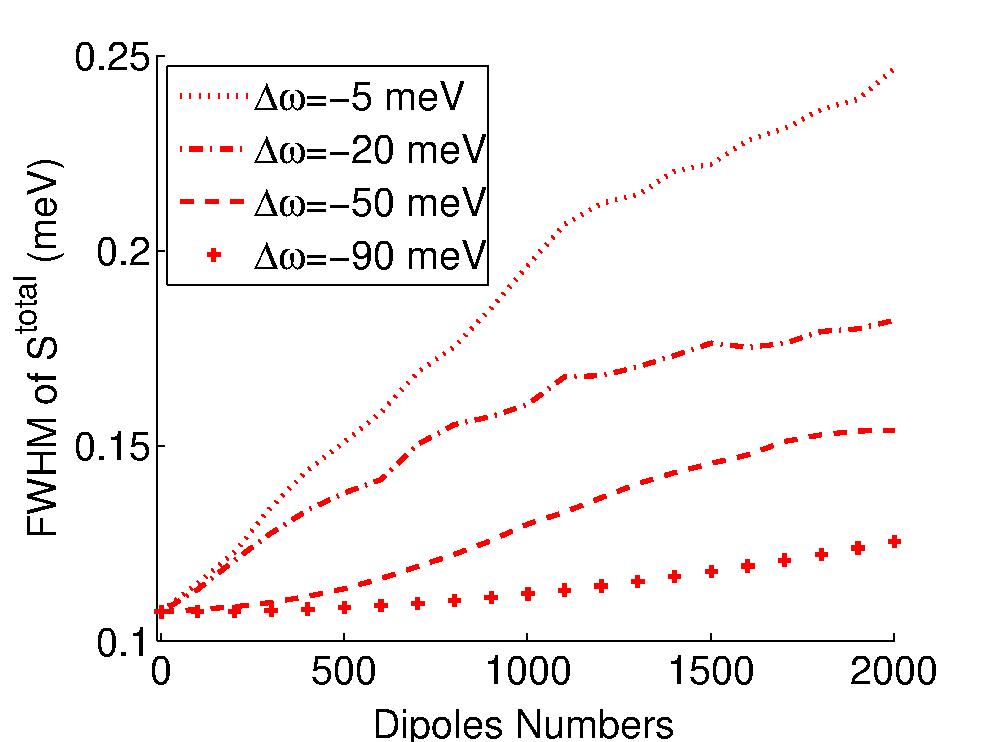
\includegraphics[width=0.46\textwidth]{./Figs/Stotalfwhm_wdrand5-90s20_gt0dot04b0dot5_qd2000_stat200}
    \label{Stotalfwhm_wdrand5-90s20_gt0.04b0.5_qd2000_stat200}}
  &
  \subfigure[ ]{
    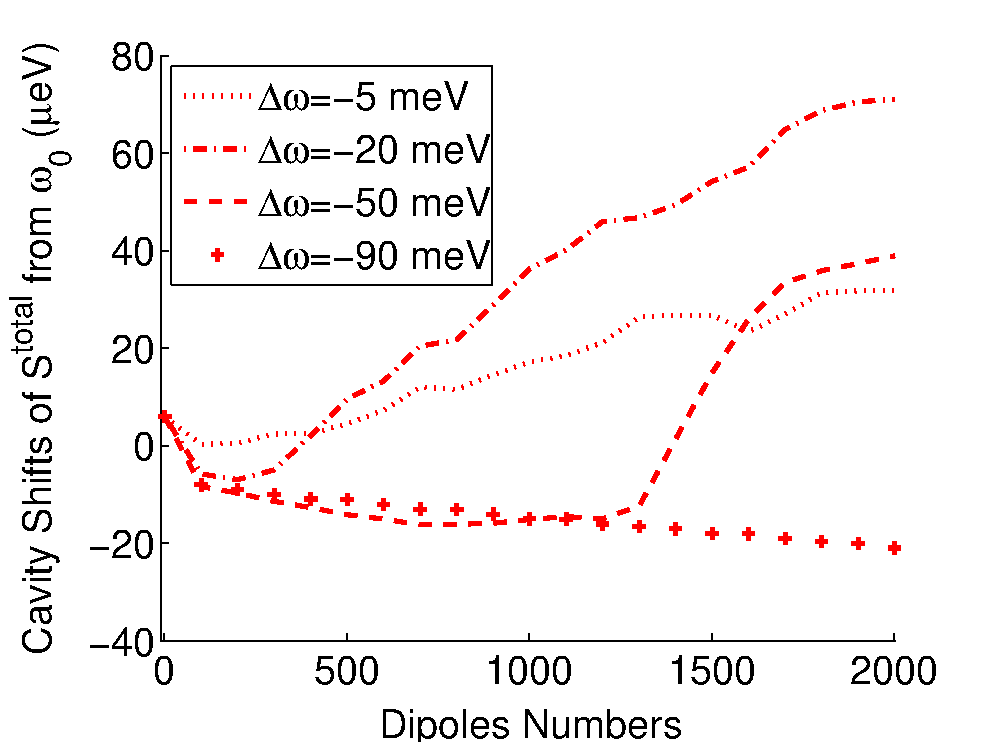
\includegraphics[width=0.46\textwidth]{./Figs/Stotalshift_wdrand5-90s20_gt0dot04b0dot5_qd2000_stat200}
    \label{Stotalshift_wdrand5-90s20_gt0.04b0.5_qd2000_stat200}}
  \\
  \subfigure[ ]{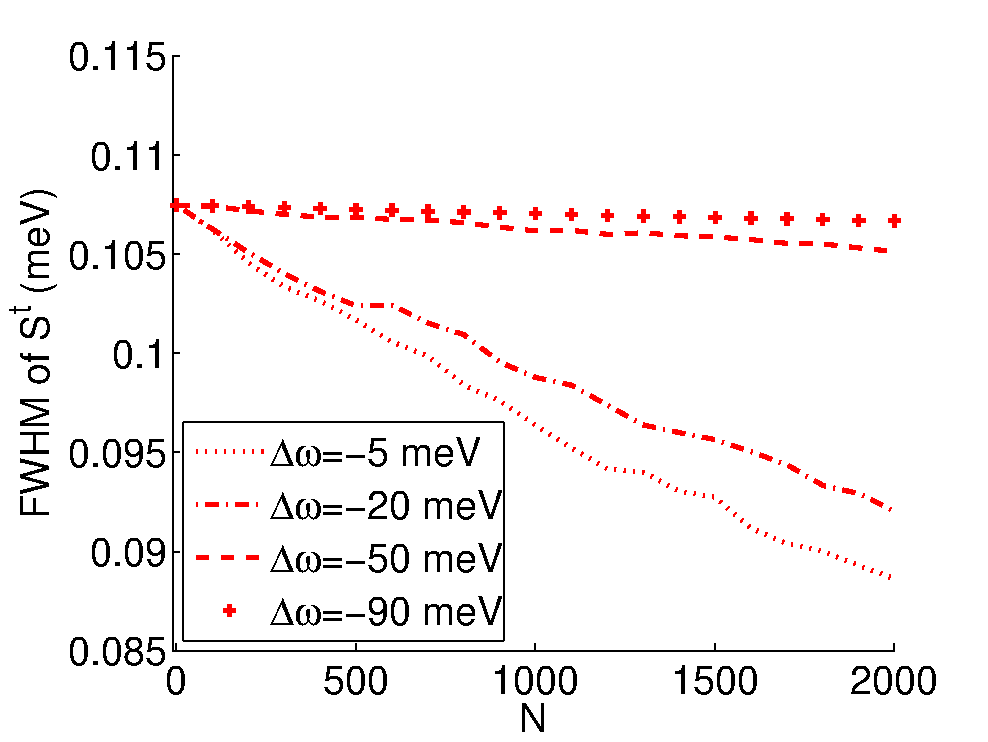
\includegraphics[width=0.46\textwidth]{./Figs/Stfwhm_wdrand5-90s20_gt0dot04b0dot5_qd2000_stat200}
    \label{Stfwhm_wdrand5-90s20_gt0.04b0.5_qd2000_stat200}}
  &
  \subfigure[ ]{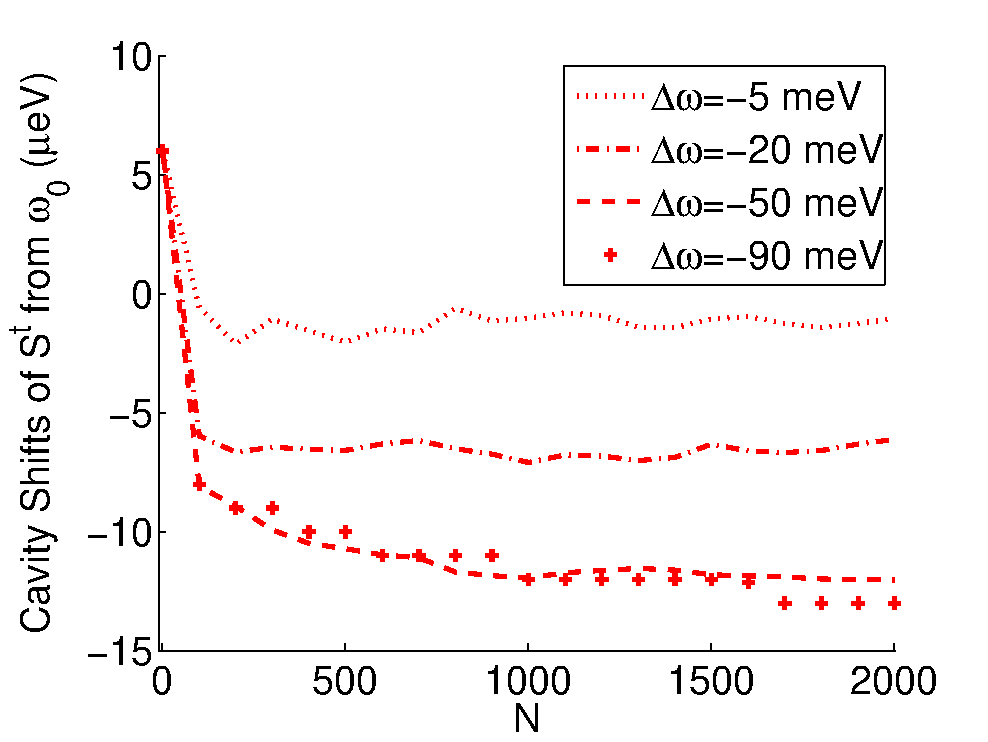
\includegraphics[width=0.46\textwidth]{./Figs/Stshift_wdrand5-90s20_gt0dot04b0dot5_qd2000_stat200}
    \label{Stshift_wdrand5-90s20_gt0.04b0.5_qd2000_stat200}}
\end{tabular}
\caption[Modification effect of different $\Delta\omega$ when $g_t=0.04$ meV.]{\textbf{FWHM and shifts of the cavity with different $\Delta\omega$ with the same $g_t=0.04$ meV.} As the doublets occur, the repulsion between doublets gives a different spectral behavior from what has been shown in Fig.~\ref{fwhm_shift_gt0.02_dw}. See text for the discussion.}
\label{fwhm_shift_gt0.04_dw}
\end{figure}


\begin{figure}[thp]%[floatfix]
\centering
\begin{center}
%\psfrag{PL}{$PL (to Max)$}
%\psfrag{omega-omega}{$\omega-\omega_c (meV)$}
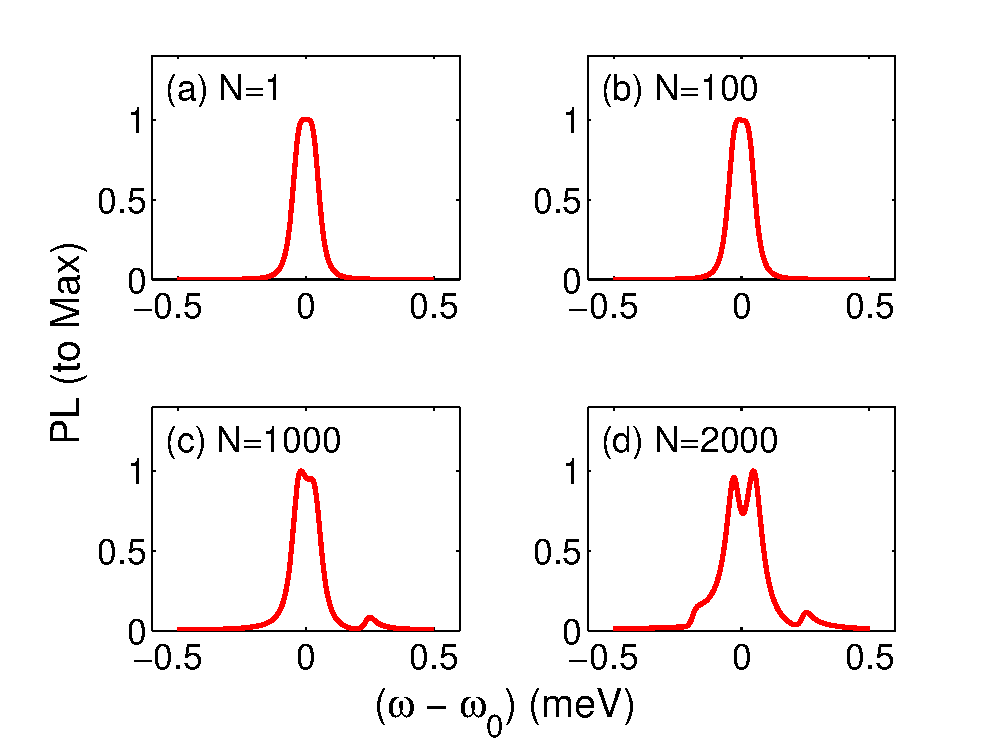
\includegraphics[width=12cm]{./Figs/spec1tNb_wd50s20_gt0dot04E0dot5_stat200} %spec_wdrand5s20_E0.2_qd2000_stat200_sam32.eps
\end{center}
\caption[Spectra sample for a cavity with a target dipole and an ensemble.]{\textbf{Cavity spectra of one set of dipoles sample ($\Delta\omega=-50$ meV, $\sigma=20$ meV) with various background dipole population $N$.} Doublets occur even though $g_t<0.5$ meV, which is the criterion of strong coupling for one-exciton cases.}
\label{spec1tNb_wd50s20_gt0.04E0.5_stat200}
\end{figure}


If the coupling strength of the target dipole is large, the cavity coupling effect takes place and the spectral behavior is different from the cases discussed above. One example with $g_t=0.04$ meV is presented in Fig.~\ref{fwhm_wdrand5s20_gt0.2-0.4_qd2000_stat200} (b) and (d) with error bars on FWHM curves. Compared with less weak coupling cases (Fig.~\ref{fwhm_wdrand5s20_gt0.2-0.4_qd2000_stat200} (a) and (c)), one can find that the cavity bandwidth is broadened much more, and the on-resonance target dipole spectrum (both the bandwidth and peak position) is largely affected by the cavity mode. To depict the interactions in the system, we present the spectral behavior with shifting $\Omega_d$ in Fig.~\ref{fwhm_shift_gt0.04_dw}. There are two features to highlight. One is that, as more background dipoles couple to the cavity, the cavity squeezes the target dipole peak (see Fig.~\ref{Stfwhm_wdrand5-90s20_gt0.04b0.5_qd2000_stat200}). The other is that the cavity spectrum splits into two peaks, and the target dipole peak is strongly repelled by the cavity peak and gives an attractive effect to the background dipoles.

Here, we explain the second feature of the spectral behavior in the case introduced in the last paragraph. Let us look in the $\Delta\omega=-50$ meV case, for example, in Figs.~\ref{Stotalshift_wdrand5-90s20_gt0.04b0.5_qd2000_stat200} and~\ref{Stotalshift_wdrand5-90s20_gt0.04b0.5_qd2000_stat200}. Initially, both cavity and target dipole peaks are equally repelled to the high frequency side because of the discrete low-frequency-side background dipoles. As more energy is transferred from the background dipole to the cavity mode, the target dipole peak is quickly repelled to the low frequency side of its original resonance; this shift also slowly repels the cavity peak to the low frequency side as more background dipoles couple to the system. Note that there is a retardation between the target dipole shift and the cavity shift. Until $N$ approaches to $1000$, both the cavity shift and the target dipole shift are basically of the same magnitude. As the cavity peak is broadened and enhanced by the background dipoles, it also starts to split into two peaks. Emerging doublets are shown in Fig.~\ref{spec1tNb_wd50s20_gt0.04E0.5_stat200} when $N=1000$. Along with the increasing $N$, the high-frequency-side peak of the cavity spectrum grows until it is larger than the low-frequency-side peak, which gives a sudden shift of cavity maximum peak position in Fig.~\ref{Stotalshift_wdrand5-90s20_gt0.04b0.5_qd2000_stat200} when $N\approx1300$. When $N\geq1400$, the high-frequency-side peak of the cavity splitting dominates the cavity spectrum (see Fig.~\ref{spec1tNb_wd50s20_gt0.04E0.5_stat200} (d) for a sample of cavity spectrum when $N=2000$). And the repulsion from the split peak of the cavity stabilizes the target dipole at a position between the two split peaks (see Fig.\ref{Stotalshift_wdrand5-90s20_gt0.04b0.5_qd2000_stat200}). For the cases with different $\Delta\omega$, a similar process happens but with different starting points of splitting depending on the effective coupling strength of the background dipoles. From the calculation above, we find that the ensemble of background dipoles can also generate evident doublets even when $g_t$ and $g_b$ are less than the critical value of $\frac{\Gamma_c}{2}$ for single excitation systems. In fact, the criterion of strong coupling for the multi-exciton coupled cavity should be used for this case~\cite{Kimble1994,Tischler2007}.


Experimentally, multilevel lasers, specially for lasers with random emitting particles in a solution with a long cavity, could be viewed as systems we discussed above. The stimulated emission from the metastable level corresponds to on-resonance dipoles, and other spontaneous emissions in the other energy interval correspond to the background dipoles. Along with the lasing process, the on-resonance emission is amplified and selected out by the optical cavity, while most spontaneous emissions either emit in random directions as optical loss or give non-radiative effects, and hence the emitting spectrum mainly corresponds to the target dipole spectrum, $S^t$. As observed in the experiments, the emitting spectrum will be squeezed if the density of gain media units or the pumping power increases within the linear optical region. Our theoretical analysis based on the scattering model above is consistent with the experimental results.


\clearpage

%\begin{figure}[h]
%\centering
%\begin{center}
%\includegraphics[width=8cm]{./Figs/GFT_ME_gb0.2gt_Gc1g_Gx0.5g_w0wd0_N_shift}
%\end{center}
%\caption{\textbf{  Cavity Spectral shifts of ME models. } Spectra are summed up from all dipole sources. For the calculation, I have made $g=g_t=0.1$ meV, $\Gamma_x=0.5g$, $\Gamma_c=g$, $g_b=0.2g_t$, $\omega_t=\omega_c-10g$. The values of $P_c$ and $P_x$ give the best fit for statistic spectra of GFT calculation with dipole number $N=[1,\,50,\, 100,\, 200,\, 1000]$, where $N=1$ means there is only one target dot in the cavity. GFT calculations are averaged from 400 samples with background dots gaussianly distributed in the range of $[-200g, \, 200g]$ around cavity resonance.  }
%\label{GFT_ME_gb0.2gt_Gc1g_Gx0.5g_w0wd0_N_shift}
%\end{figure}

%\begin{figure}[h]
%\centering
%\begin{center}
%\includegraphics[width=8cm]{./Figs/GFT_ME_gb0.2gt_Gc1g_Gx0.5g_w0wd0_N_width}
%\end{center}
%\caption{\textbf{  Cavity Spectral widths of ME models. } Spectra are summed up from all dipole sources. For the calculation, I have made $g=g_t=0.1$ meV, $\Gamma_x=0.5g$, $\Gamma_c=g$, $g_b=0.2g_t$, $\omega_t=\omega_c-10g$. The values of $P_c$ and $P_x$ give the best fit for statistic spectra of GFT calculation with dipole number $N=[1,\,50,\, 100,\, 200,\, 1000]$, where $N=1$ means there is only one target dot in the cavity. GFT calculations are averaged from 400 samples with background dots gaussianly distributed in the range of $[-200g, \, 200g]$ around cavity resonance.  }
%\label{GFT_ME_gb0.2gt_Gc1g_Gx0.5g_w0wd0_N_width}
%\end{figure}


%     \begin{singlespacing}
%     \begin{Listing}[h]
%     \fileinsmall{Examples/connectToVM.txt} \caption[Excerpt from
%     \texttt{StateDumperThreads.java}]{Excerpt from \texttt{StateDumperThreads.java},
%     showing how to connect to a second virtual machine executing the target code.  In
%     this example, the target class is referenced by \texttt{javaClassName}.  The JPDA
%     classes can be accessed by including the \texttt{tools.jar} archive in the program's
%     classpath; this archive is found in the Java installation's \texttt{lib} directory}
%     \label{list:connectToVM}
%     \end{Listing}
%     \end{singlespacing}
%
%
%     \begin{figure}[h]
%     \begin{singlespacing}
%     \centering
%         \subfigure[Specification of binary \texttt{next} relation]{
%             \begin{minipage}{100pt}
%                 \filein{Examples/smallA.txt}
%             \label{fig:smallBinary}
%             \end{minipage}}
%         \hspace{0.25in}
%         \subfigure[Implementation of binary relation in (a)]{
%             \begin{minipage}{100pt}
%                 \filein{Examples/smallB.txt}
%             \label{fig:smallBinaryCode}
%             \end{minipage}}
%         \hspace{0.25in}
%         \subfigure[Specification of ternary \texttt{next} relation]{
%             \begin{minipage}{100pt}
%                 \filein{Examples/smallC.txt}
%             \label{fig:smallTernary}
%             \end{minipage}}
%     \caption[Sample specification and implementation]{Sample specification and
%     implementation of a binary relation; sample specification of a ternary relation}
%     \end{singlespacing}
%     \end{figure}
%
% \section{High-Q Cavity Mode Calculation}\label{sec:cavity}

\subsection{Definition of Terms}\label{sec:termDefn}

    The following terms...:

    \begin{Ventry}{\boldmath $\operatorname{arity}(r_i)$ \unboldmath}

        \boldmath \item[$scope$] \unboldmath
        The maximum number of objects...

        \boldmath \item[$R$] \unboldmath
        The number of relations...

        \boldmath \item[$r_i$] \unboldmath
        The $i^\text{th}$ relation in the specification, $1 \le i \le R$.

        \boldmath \item[$\operatorname{arity}(r_i)$] \unboldmath
        The arity of relation $r_i$...

        \boldmath \item[$N$] \unboldmath The total number...

        Given the calculated arities of a particular specification's relations, and the scope at
        a specific breakpoint, Equation~\ref{equation:N} can be used to determine $N$.
        \begin{equation}\label{equation:N}
        N = S \times scope + \sum_{i=1}^R scope ^ {arity(r_i)}
        \end{equation}

    \end{Ventry}



    The combined complexity of all four steps is
    \begin{equation*}
        O(N) + O(nN) + O(N^2) + O(F)
    \end{equation*}
    Again, these steps are completed once for every breakpoint in the target program's
    execution; therefore, the overall upper bound becomes
    \begin{equation*}
    \begin{split}
        & b \times O(N) + b \times O(nN) + b \times O(N^2) + b \times  O(F) \\
                   = ~ & O(bN + bnN + bN^2 + bF)
    \end{split}
    \end{equation*}


    The vector [$x_0$  $x_1$] represents the two possible atoms of type
    \texttt{X}.  With our naming scheme, $x_0$ represents \texttt{X\_0} and $x_1$
    represents \texttt{X\_1}.
    The binary relation itself is represented by a two-dimensional bit matrix where a 1 in
    position [$i$,$j$] means that there is a mapping between the $i^{th}$ atom of \texttt{X}
    and the $j^{th}$ atom of \texttt{Y}:

    \begin{gather*}
    \begin{bmatrix}
      r_{00} & r_{01} \\
      r_{10} & r_{11} \\
    \end{bmatrix} \quad
    \begin{bmatrix}
      \texttt{X\_0->Y\_0} & \texttt{X\_0->Y\_1} \\
      \texttt{X\_1->Y\_0} & \texttt{X\_1->Y\_1} \\
    \end{bmatrix}
    \end{gather*}
    \medskip

    Now, consider a fact stating that relation \texttt{r} is total, i.e.,

    \begin{center}
    \texttt{all x :~X | some y :~Y | x.r = y}
    \end{center}

    The CNF formula for our example fact, in scope~2, is
    \begin{equation*}
    \begin{split}
    & \neg(((x_0 \wedge r_{00}) \vee (x_1 \wedge r_{10})) \wedge \neg((x_0 \wedge r_{01})
    \vee (x_1 \wedge r_{11}))) \wedge \\ &\neg(\neg((x_0 \wedge r_{00}) \vee (x_1 \wedge
    r_{10})) \wedge ((x_0 \wedge r_{01}) \vee (x_1 \wedge r_{11})))
    \end{split}
    \end{equation*}
    \medskip

    Table~\vref{fig:fullRunTimesAllPhases} contains...

    \begin{singlespacing}
    \begin{center}
    \begin{threeparttable}
    \caption{Running times for each phase and total running time of Embee}
    \label{fig:fullRunTimesAllPhases}\begin{small}
        % Table generated by Excel2LaTeX from sheet 'Embee'
        \begin{tabular}{|l|c|c|c|c|c|c|c|} \hline

        \multicolumn{3}{|c|}{Test Case} & \multicolumn{ 5}{c|}{Running Time (m:ss)} \\ \hline

        \multicolumn{1}{|c|}{Object} & & Number of & & & \multicolumn{2}{c|}{ Phase 3} &  \\  \cline{6-7}

        \multicolumn{1}{|c|}{Model} & \raisebox{1.5ex}[0pt]{Scope} & Breakpoints &  \raisebox{1.5ex}[0pt]{Phase 1} & \raisebox{1.5ex}[0pt]{Phase 2} &   First 16 &   Last 4 &  \raisebox{1.5ex}[0pt]{Total} \\

        \hline
            List  &  20 &  20           &  0:07 &  0:32 &  0:12 &  06:39 & 07:30 \\
        \hline
            Graph &  20 &  19\tnote{a}  &  0:07 &  1:27 &  0:35 &  44:10 & 46:19 \\
        \hline
            Tree  &  20 &  20 &  0:04   &  1:20 &  0:21 &  06:04 &  07:49 \\
        \hline
        \end{tabular}
    \begin{tablenotes}
    \item[a] Breakpoints occur after the addition of each edge, i.e., the first
    breakpoint does not occur until the second node is added.
    \end{tablenotes}
        \end{small}
    \end{threeparttable}
    \end{center}
    \end{singlespacing}


    ...upper bound on Embee's performance:

    \begin{numcases}{\text{upper bound is}}
        O(bN^2) & if $scope \leq 16$ \notag \\
        O(bF)   & if $scope > 16$ \notag
    \end{numcases}

